%%%%%%%%%%%%%%%%%%%%%%%%%%%%%%%%%%%%%%%%%%%%%%%%
% BOZZA PER TESI DI LAUREA IN LATEX
%%%%%%%%%%%%%%%%%%%%%%%%%%%%%%%%%%%%%%%%%%%%%%%%

%\documentclass[12pt,titlepage]{book}
\documentclass[a4paper,twoside,12pt]{article}
\usepackage[british]{babel}
\usepackage{gensymb}
\usepackage[toc,page]{appendix}
%\usepackage{graphics}
%\usepackage{url,amsfonts,epsfig}
%\usepackage[applemac]{inputenc} %comando per le lettere accentate se usate mac  
\usepackage[utf8]{inputenc} % comando per le lettere accentate se usate pc  
\usepackage[nottoc]{tocbibind}
\usepackage{unipitesi}
\usepackage[font=small]{caption}
\usepackage{subcaption}
\usepackage{hyperref}
\usepackage{textcomp}
\usepackage{graphicx}
\usepackage{amsmath}
\usepackage{amssymb}
\usepackage{xcolor}
\usepackage{verbatim}
\graphicspath{ {Images/} }

\hypersetup{
colorlinks=true,
linkcolor=blue,
urlcolor=blue
}
\urlstyle{same}

\pagestyle{headings}

\definecolor{dred}{RGB}{200,0,0}
\definecolor{dblue}{RGB}{0,0,200}

%\title{\textsc{Analysis of performance of ATLAS experiment Phase 2 inner tracker}}
%\author{Federico Massa}

\begin{document}

%%%% Opzione per interlinea 2
%%%\baselineskip 18pt

%\maketitle

\titolo{\textit{Studio delle prestazioni dei} \\
			\textit{ layout di ITk nelle misure di $H\rightarrow ZZ^{*}\rightarrow 4\mu$ }}
\laureando{Federico Massa} 
\corsodilaureamagistrale{Fisica} 
\relatore[Prof.]{Giorgio Chiarelli} 
%\secondorelatore[Prof.]{prof2} s
%\controrelatore[Prof.]{prof3} 
\annoaccademico{2015-2016} 
\data{data}
\maketitle


\tableofcontents
%%\listoffigures
%%\listoftables
\newpage

\begin{abstract}
La fase di High Luminosity LHC offrirà nuove opportunità per esplorare eventi estremamente rari, ed in particolare per studiare la fisica e le proprietà del bosone di Higgs.
L’esperimento ATLAS, per sfruttare al massimo questa possibilità, sostituirà l’Inner Tracker  all’attuale Inner Detector.
A causa dell'elevato numero di eventi di pileup ($>200$) previsti, il tempo richiesto dalla simulazione Monte Carlo risulta proibitivo. E’ stato, pertanto, sviluppato un metodo ad-hoc che permette di simulare solo le regioni di interesse in modo accurato, confrontando differenti configurazioni del rivelatore. In questo studio presentero' i risultati ottenuti relativamente al canale\\ {$H\rightarrow ZZ^*\rightarrow 4\mu$}
\end{abstract}

\newpage

\section{Introduction} \label{sec:introduction}
The Large Hadron Collider (LHC) accelerator is scheduled to be upgraded in two different stages: the first one will begin after the end of Run 2 during the Long shutdown 2 (LS2) in 2019-2020; the second one will start at the end of Run 3 during the Long shutdown 3 (LS3) in 2024-2026 (Fig.\ref{fig:HLLHC_Plan}). The latter upgrade stage will lead to what is known as High-Luminosity LHC (HL-LHC) during which the
luminosity will reach the maximum value of $7.5 \times 10^{34}\ cm^{-2}s^{-1}$, corresponding to approximately $3000\ fb^{-1}$ during ten years of data taking. \\

\begin{figure} [h]
	\includegraphics[width=\textwidth]{HLLHC_Plan}
	\caption{LHC/HL-LHC Plan as scheduled in 2015\cite{scoping}.}
	\label{fig:HLLHC_Plan}
\end{figure}

HL-LHC will allow to study new physics processes, such as extra dimensions or the ones predicted by SUSY models, as well as improve Standard Model measurements. In particular, Higgs boson 
couplings are expected to be measured with a precision between 5\% and 30\%\cite{loi}. Thanks to the increased luminosity, it will be possible to observe the Higgs boson in rare
channels such as  $H \rightarrow \mu\mu$, vector boson 
fusion production of $H \rightarrow \gamma\gamma$ and $H \rightarrow \tau\tau$, associated production $t\bar{t}H$ with $H \rightarrow \gamma\gamma$, as well as Higgs self couplings
such as in $HH \rightarrow \tau\tau b b$, $HH \rightarrow \gamma\gamma b b$.\\

By the end of Run 3, ATLAS detector will be using 15-20 years old components. In particular,
the highly irradiated Inner Detector pixels and strips will have reached the end of their
lifetime and the transition radiation tracker will reach 100\% occupancy at that luminosity. Thus, the Inner Detector will have to be completely substituted by the Inner Tracker (ITk), which will
have to guarantee the same or an improved performance in the harsh conditions of HL-LHC while maximizing the acceptance. At the design luminosity, the expected number of in-time pileup events will be $<\mu > = 200$, a much
higher value than the one expected at the end of Run 3 ($<\mu > = 80$) and even more if 
compared to the current one ($<\mu > = 35$??), introducing new challenges in the pattern
recognition. The increase of the number
of collisions per bunch crossing leads to new requirements on the front-end electronics, trigger and data acquisition system that cannot be met by the current apparatus, thus leading to a 
substantial upgrade of the electronics. Moreover, in the Reference Scenario of the Scoping Document\cite{scoping} the geometrical acceptance of ATLAS detector is increased with respect to 
the current one thanks to the extension of the $|\eta|$ coverage to $4.0$, which requires either the substitution (such as in the case of ITk) or the addition of new detectors (muon chambers,
calorimeter system). \\

Other than detector and hardware upgrades, HL-LHC will require software upgrades to meet the needs of the upgraded detectors, handle large event samples and adapt to multi-processor
architectures. To deal with the simulation size and time requirements it will be necessary to mix fast simulation techniques (using detector parametrisations) with full simulation at event level.


\subsection{Coordinate system - perigee parameters definition - maybe in appendix}


\newpage

\section{Detector} \label{Detector}

\begin{figure} [h]
	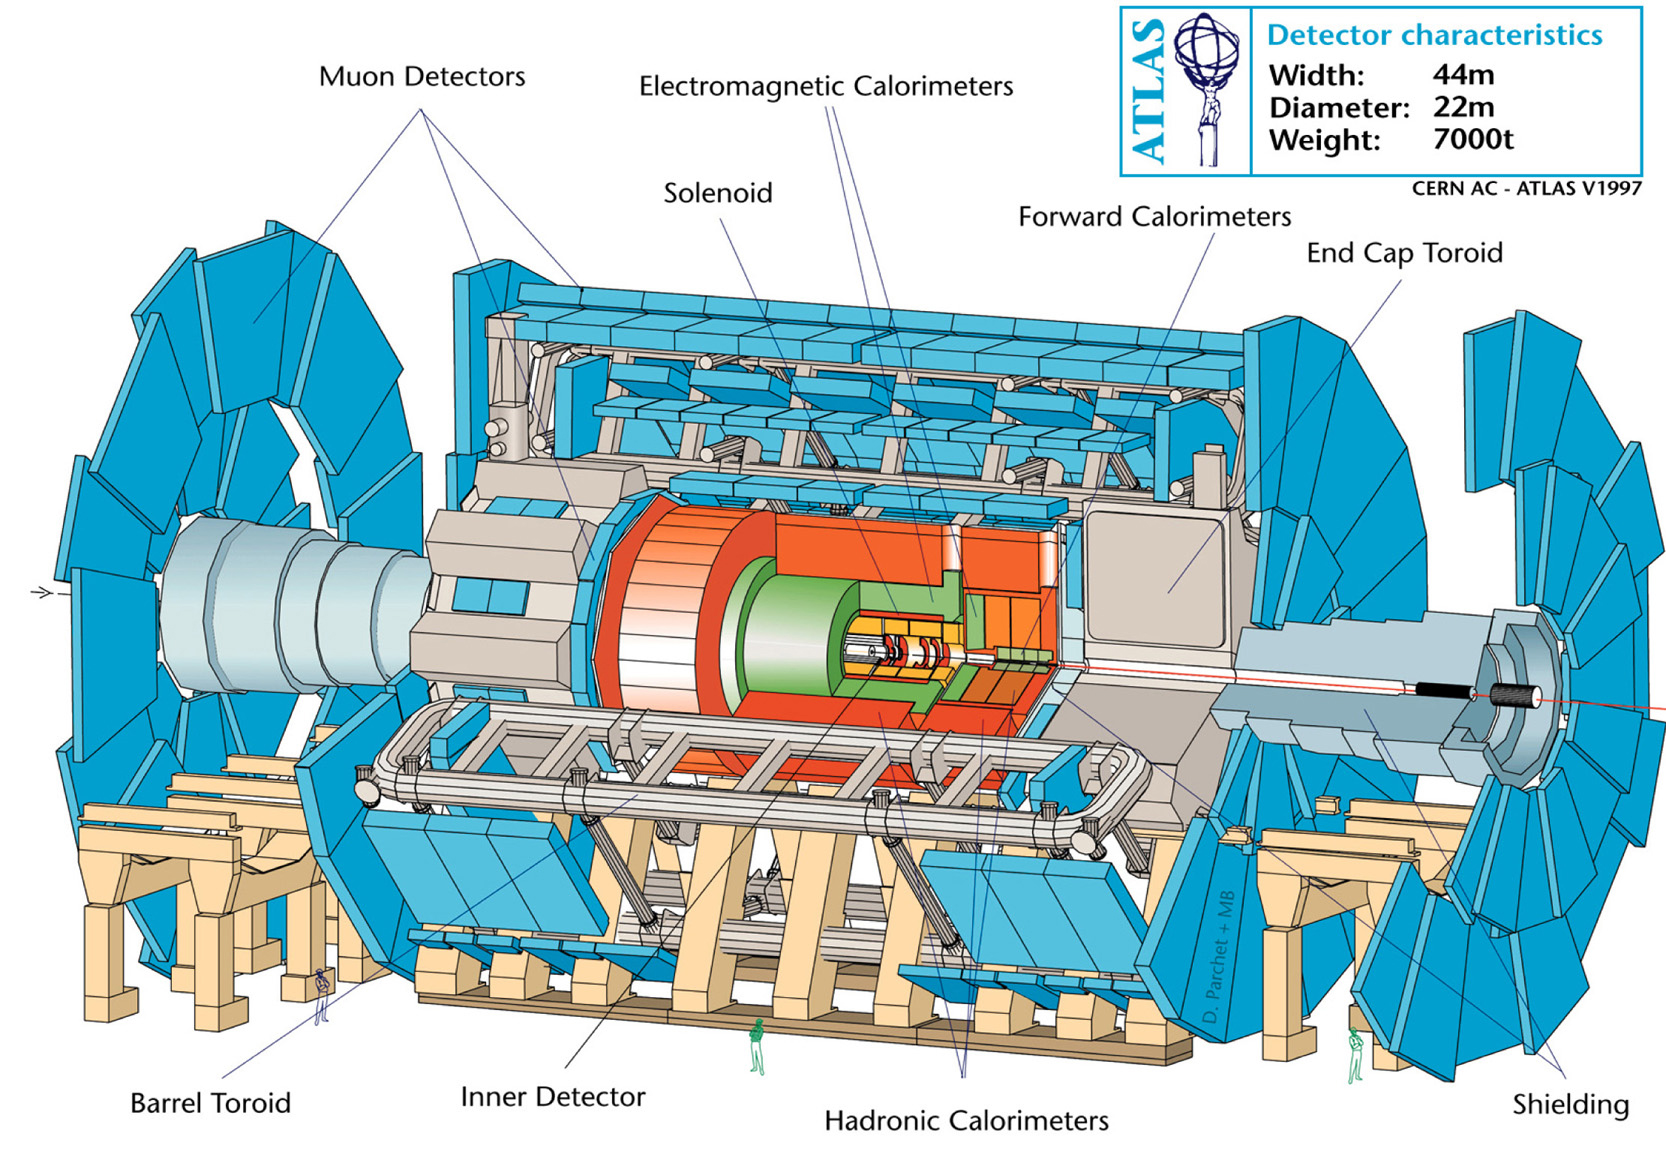
\includegraphics[width=\textwidth]{atlasdet}
	\caption{Current ATLAS detector.}
	\label{fig:current_atlasdet}
\end{figure}

This section briefly describes the current experimental apparatus, shown in Figure \ref{fig:current_atlasdet}, and the reasons as to why it cannot withstand the conditions of HL-LHC.
\smallskip
ATLAS detector is currently composed by the following components:
\begin{itemize}
\item a \textbf{magnet system}
\item an \textbf{inner detector}
\item an \textbf{electromagnetic calorimeter}
\item an \textbf{hadronic calorimeter}
\item a \textbf{muon spectrometer}
\item a \textbf{trigger system}
\item a \textbf{data acquisition system (DAQ)}
\end{itemize}

In the following sections these elements are briefly described, outlining the main upgrades that will be applied for HL-LHC. 

\subsection{The magnet system}\label{sec:magnet}

\begin{figure} [h]
	\centering
	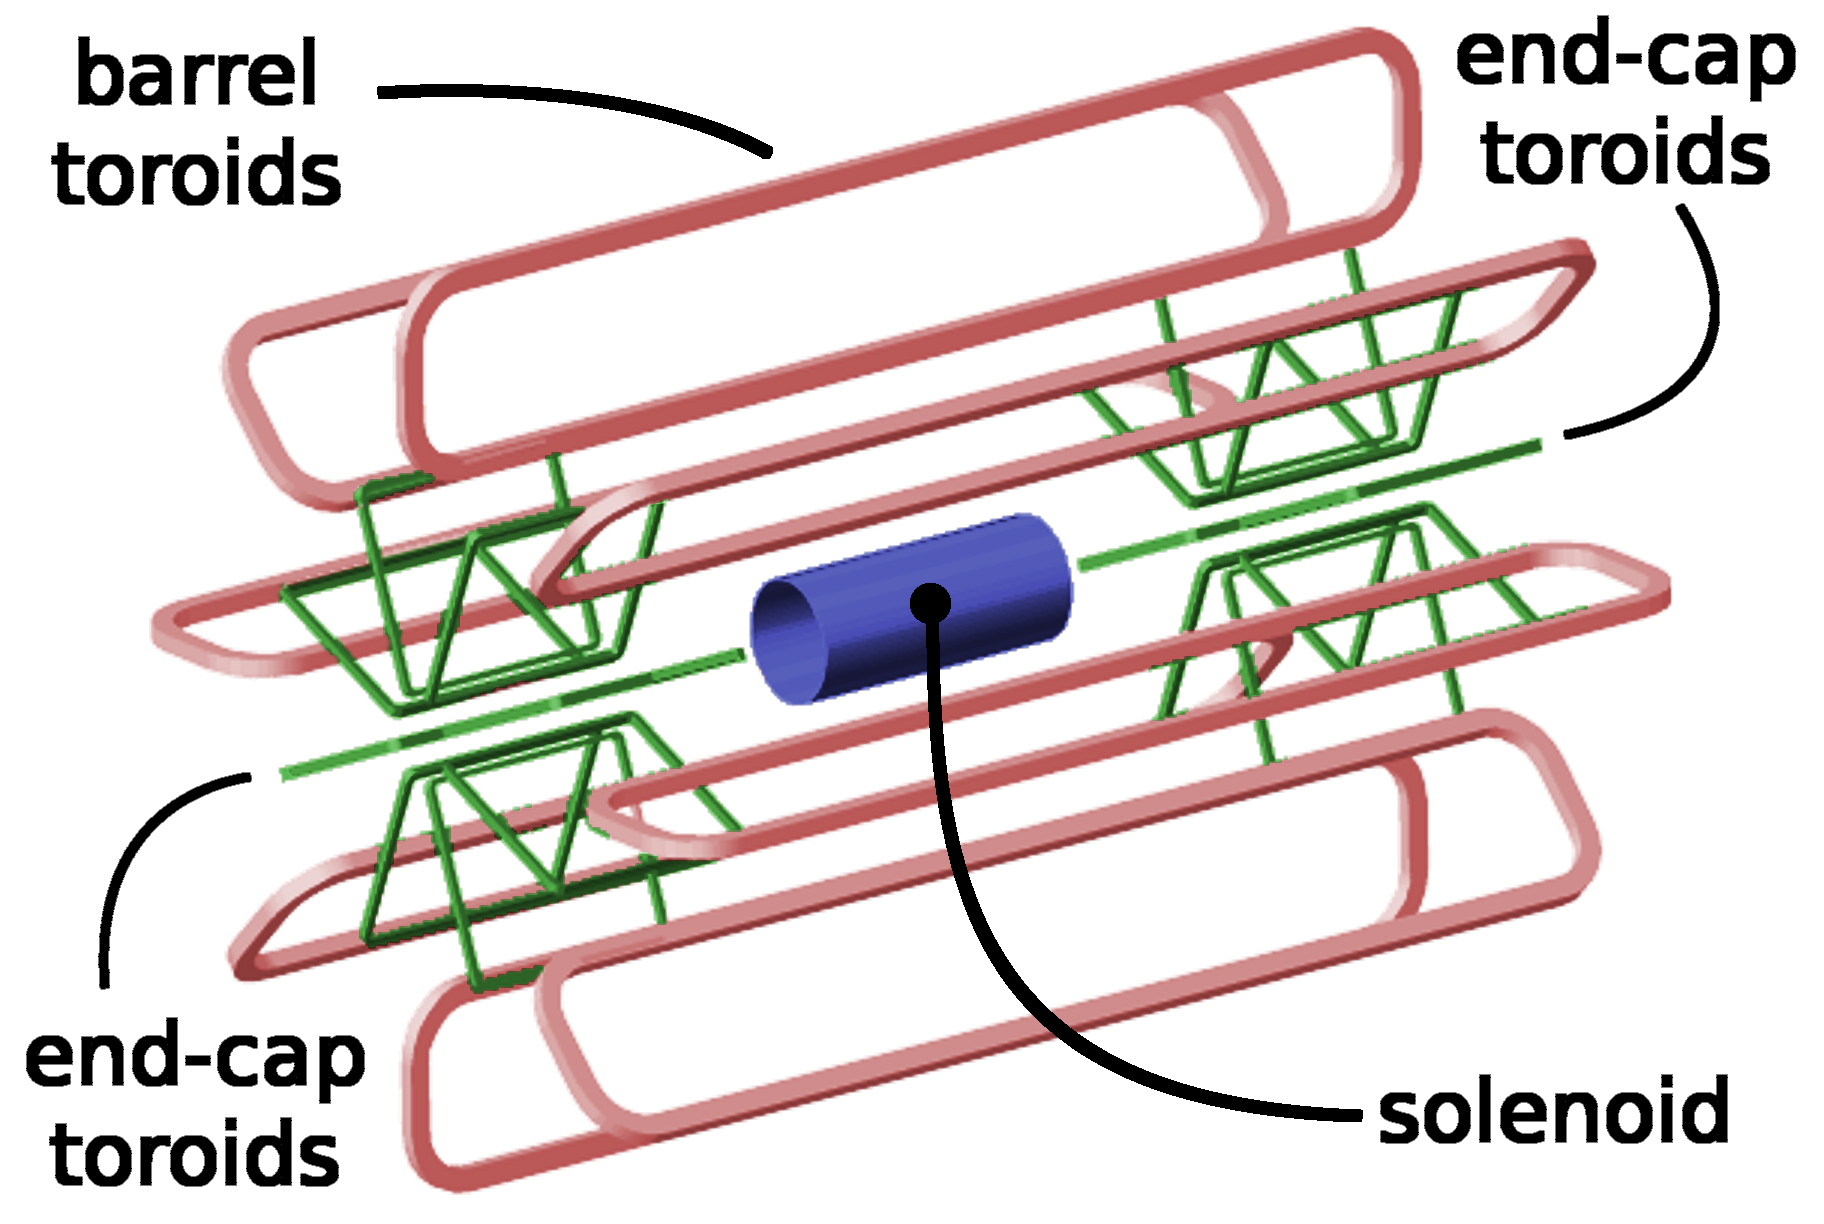
\includegraphics[scale=0.13]{magnetSystems}
	\caption{ATLAS magnet system\cite{magnet_system_picture}.}
	\label{fig:magnet_system_picture}
\end{figure}

The current magnet system (Fig.\ref{fig:magnet_system_picture}) comprises four superconducting magnets\cite{magnet_system}, for charged particles bending and momentum measurement in the $8000\ m^3$ volume of the apparatus.\\

The \textit{Central Solenoid Magnet} encloses the tracking volume and provides a $2\ T$ magnetic field and minimal thickness in order to reduce the degradation of photon and electron energy resolution in the subsequent calorimeter layers.\\

The \textit{Barrel} and \textit{Endcap Toroids} provide a tangential magnetic field of about $1\ T$ for the muon detectors, both in the radial and the forward region.\\

As the current magnet system already fulfils HL-LHC requirements, it will not require an
upgrade. [ref? NON SE NE PARLA NEL LOI/SCOPING]

\subsection{The Inner Detector}

\begin{figure} [h]
	\includegraphics[width=\textwidth]{IDLayout}
	\caption{ATLAS Inner Detector layout\cite{Aad:2008zzm}. IBL is not shown in this layout.}
	\label{fig:IDLayout}
\end{figure}

The ATLAS \textbf{Inner Detector} (ID), whose layout is shown if Fig.\ref{fig:IDLayout}, is designed to measure the momentum of the
charged particles tracks with $p_{T}$ larger than a typical threshold of $500\ MeV$ and 
within $|\eta| < 2.5$, identifying both primary and secondary vertices\cite{Aad:2008zzm}. \\

The ID is contained in a cylindrical envelope (with the axis along the z-axis) that extends
$\pm\ 3512\ mm$ in length and $1150\ mm$ in radius. The whole system is placed inside
a solenoid magnet which produces a field parallel to the beam line of $2\ T$(see sec.\ref{sec:magnet}). The ID is composed by three sub-detectors: the innermost section provides
high resolution pattern recognition using \textit{silicon pixel layers}, the middle one consists of stereo pairs of \textit{silicon microstrip} (SCT) layers and the outermost one consists of the \textit{Transition Radiation Tracker} (TRT). During 2014 ATLAS upgrade, the \textit{Insertable B-Layer} (IBL), a fourth pixel barrel layer, was added to avoid the decrease of performances after the luminosity upgrade. \\

Each one of these detectors is subdivided into a \textit{barrel} region, in which the sensor modules 
are organized tangentially with respect to a circle around the beam axis and an \textit{end-cap} region, in which they are placed perpendicularly with respect to the beam axis, producing
a disk resemblant shape.\\

The \textit{pixel} barrel layout consists of 3 layers placed at approximate radii $50.5\ mm$, $88.5\ mm$ and $122.5\ mm$ with respect to the beam 
axis. A fourth layer called \textit{Insertable B-Layer} (IBL) was added during the LS1 as the
innermost pixel layer at radius $32.7\ mm$. In the end-cap region, three disks per side were chosen,
at z position respectively $495\ mm$, $580\ mm$, $650\ mm$. \\

The \textit{SCT} barrel layout consists of four layers at radii $300\ mm$, $373\ mm$, $447\ mm$ and $520\ mm$. The end-cap region is instead composed by 9 disks per side with variable
inner radii and z-position ranging from $850\ mm$ to $2720\ mm$. \\

The \textit{TRT} barrel layout is formed by straws parallel to the beam axis (GIUSTO?) at radii from $563\ mm$ to $1066\ mm$,
while the end-cap region consists of radially wound straws with z ranging from $850\ mm$ to 
$2710\ mm$. 

\subsubsection*{Pixel and SCT} (DIFFERENZE CON TDR: dimensioni diverse dei singoli pixel)

The pixel and SCT sensors are designed to maintain their performance during the detector
lifetime at nominal luminosity\cite{Aad:2008zzm}. As the integrated radiation dose has significant consequences
on these sensors, they are operated at a temperature between $-10\ ^{\circ}C$ and $-5\ ^{\circ}C$.\\

\textit{Pixel sensors} of the Run 1 ID (thus excluding IBL) are $250\ \mu m$ thick detectors which are mounted on oxygenated n-type wafers, with the pixel on the $n^+$ side(??). About 90\% of the pixel on a sensor have a nominal 
size of $50 \times 400\ \mu m^2$, while the rest are $50 \times 600\ \mu m^2$ large and are placed
at the front-end chips on a module. There are a total of 1744 identical pixel sensors(modules??) with an external dimension of $19 \times 63\ mm^2$, each composed by 47232 pixels. For reasons of space, there are four ganged pixels on each column of the front-end chip, thus resulting in a total of 46080 readout channels. \\

\textit{IBL pixels} are, instead, $50 \times 250\ \mu m^2$ large to 
ensure a highly precise measurement of the coordinates near the interaction point\cite{IBL}. Two 
different technologies have been implemented in the central and forward IBL region, which
results in a different sensor thickness and chip size.\\

The \textit{SCT} consists of a total of 15912 sensors with thickness $285\ \pm\ 15\ \mu m$. Every sensor consists of 768 strips of $12\ cm$ length, with average pitch of $80\ \mu m$.
On each SCT module there are two back-to-back sensors with a relative angle of $40\ mrad$,
which allows the extraction of a second coordinate.

\subsubsection*{TRT}
The basic elements of \textit{TRT} consist of $4\ mm$ diameter tubes\cite{Aad:2008zzm}. For both the barrel
and end-cap sections, the anodes are made of $31\ \mu m$ diameter, $\pm\ 71.2\ cm$ 
active length tungsten wires 
connected to the front-end electronics and grounded. The wires are carefully aligned within
the straw, with a maximum tolerance of $300\ \mu m$. The barrel section contains about 
50000 straw tubes, whereas the end-cap contains approximatively 320000,
for a total of 420000 electronic channels\cite{ATLAS:1997ag}. This detector typically provides
an almost continuous tracking of the particles traversing it, with an average of 36 measurements per track.\\

\bigskip
The upgrade of the ID is the main focus of this thesis and will be covered in sec.\ref{sec:ITkLayouts}.


\subsection{Calorimeter system}

ATLAS experiment  relies on an electromagnetic and an hadronic calorimeter for the identification and the measurement of physical quantities of photons, electrons, hadrons and jets. 
Both compartments are divided into a central and a forward region (Fig.\ref{fig:current_Cals}).

\begin{figure} [h]
	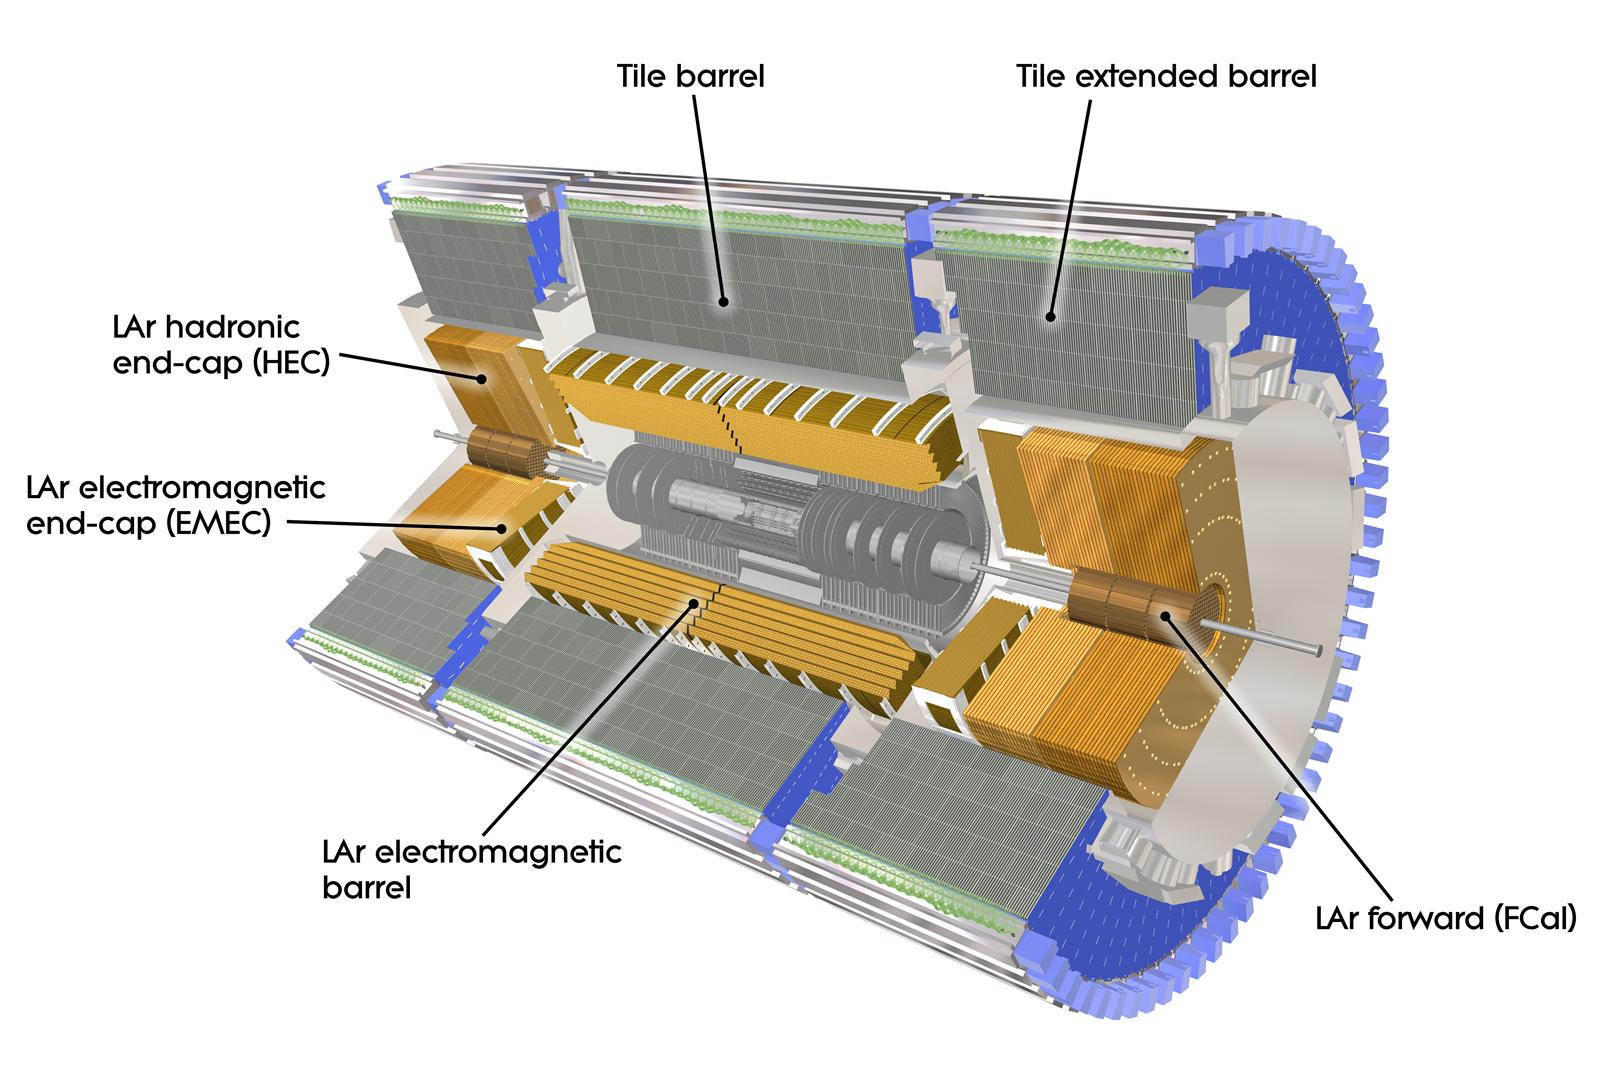
\includegraphics[width=\textwidth]{current_Cals}
	\caption{ATLAS Calorimeter System.}
	\label{fig:current_Cals}
\end{figure}

\subsubsection*{Liquid Argon Calorimeters}\label{sec:LAr}
Several components of the ATLAS calorimeter use liquid Argon (LAr) as active medium\cite{current_EMCal}. The electromagnetic barrel and endcap (EMEC) are entirely made up this way, but also the Hadronic Endcap Calorimeter (HEC) and the Forward Calorimeter (FCal). \\[2pt]
The \textbf{electromagnetic calorimeter} uses lead as absorber and is designed to trigger on and to provide precision measurements of electrons, photons, jets, and missing $E_T$ .
The full cryostat of the \textit{barrel section} is $6.8\ m$ long, with the inner and outer radius being respectively $1.15\ m$ and $2.25\ m$ and ranges in $|\eta|$ from 0 to 1.7.  The \textit{endcap section} consists of two concentric wheels, the larger one ranging in $|\eta|$ from 1.4 to 2.5, the smaller from 2.5 to 3.2. In addition, a \textit{presampler} layer has been inserted behind the cryostat wall to allow measurement correction due to losses in the upstream material. 
%The amount of inactive material due to the solenoid
%accounts for $0.63\ X_0$ and, as cited in Sec.\ref{sec:magnet}, has been optimized. 
Detailed simulations based on the response to high energy photons and electrons have
measured the thickness of the calorimeter to be about $24\ X_0$ in the barrel and $26\ X_0$ in the endcap. Each section is physically divided into towers which produce the signal and are so responsible
for the granularity of the calorimeter.
High granularity is especially required in the central regions, where it reaches the value of 
$\Delta\eta\ \times\ \Delta\phi\ =\ 0.025\ \times\ 0.025$, sometimes allowing to combine the information
coming from the inner detector to improve rejection power.
\begin{comment}
 In this region it is possible to combine the signal of the calorimeter with the information coming from the inner detector to improve the rejection power of $\pi_0$ against photons. Indeed, granularity is less and less relevant to the overall performance with increasing $|\eta|$. 
\end{comment}
Hermeticity is also a very important feature for the measurement of missing $E_T$ and has been maximized using a transition gap between the barrel and endcap cryostats of 95 mm. \\

\textbf{HEC}\cite{hec} is a sampling calorimeter with copper absorber plates and consists of two wheels of outer radius $2.03\ m$, made of 32 identical modules. It ranges in $|\eta|$ from 1.4 to 3.2 and every half of it shares the cryostat with the EMEC and FCal. \\[2pt]

\textbf{FCal} has to cope with a high level of radiation, which makes it a particularly challenging detector. 

\begin{comment}
To avoid an excessive neutron albedo in the central cavity the detector is actually recessed by 
$1.2\ m$ with respect to the frontal face of the electromagnetic calorimeter. FCal is a high density mixed copper-tungsten calorimeter and covers the range of $3.0\ < |\eta|\ <\ 4.9$. 
\end{comment}

 The high material density employed allows to reach the required $9.5\ \lambda$ in a reduced space and to minimize the endcap calorimeter pileup signal.  \\[2pt]

\subsubsection*{Hadron Tile calorimeters}
The main requirement for the \textbf{Tile Calorimeter} is to reconstruct the energy of the jets produced in the collisions and, due to the high center-of-mass energy at LHC, it has to assure 
high performances in a wide range of energies. Thanks to the use of an extended barrel, the HEC and the FCal (see Sec.\ref{sec:LAr}), it also provides a good $p_T^{miss}$ reconstruction.\\

The Tile calorimeter is a sampling calorimeter composed by alternated layers of scintillating tiles as active medium and steel as an absorber. The signal is carried out from each module using optical fibres, which can run through the layers thanks to the laminated structure of the calorimeter. It is segmented and provides a resolution of
$\Delta\eta \times \Delta\phi\ = 0.1 \times 0.1$.\\
The Tile Calorimeter is made up of one barrel ($5.64\ m$ long) and two extended barrel ($2.91\ m$ long) parts, with a gap of $60\ cm$ in between. It consists of a cylindrical structure of inner radius $2.28\ m$ and $4.23\ m$. The barrel covers the region $0\ <\ |\eta|\ <\ 1.0$ whereas the extended barrel covers the region $0.8\ <\ |\eta|\ <\ 1.7$. The overlap region from 0.8 to 1.0 is
occupied by the Intermediate Tile Calorimeter (ITC).\\

\subsubsection*{Upgrade of the electromagnetic calorimeter}

The performance required by HL-LHC barrel electromagnetic calorimeter is the same as the current one, thus it does not need to be upgraded. In contrast to that, the FCal performances will be degraded by the conditions of HL-LHC. In the Reference Scenario of the ATLAS Scoping Document\cite{scoping} the replacement of the current FCal with a high-granularity Small-Gap Forward Calorimeter (sFCal) is foreseen, which is superior to the current one in terms of resolution and size of LAr gaps. These latter are designed to be smaller than the current in order to reduce the risk of formation of Argon bubbles, due to the high energy release. (??) The improvement in granularity would be also required by the extension in $|\eta|$ of the Inner Detector in the aforementioned scenario (??). Also, the addition of a High Granularity Timing Detector (HGTD) is planned, which will be hopefully installed in front of the LAr Calorimeter endcaps and will be needed to reduce the (OUT-OF-TIME?) pileup signal. It will cover the range $2.4\ <\ |\eta|\ <\ 4.3$ and it will measure the arrival time of charged particles, assigning them to different collision vertices. The readout electronics will also need to be upgraded due to insufficient radiation tolerance and poor performance with respect to that necessary for the foreseen trigger upgrade. In the Middle and Low cost 
scenarios, on the contrary, no upgrades in the endcap and forward region are foreseen, unless the risk of formation of Argon bubbles is considered too high, in which case a MiniFCal will be installed in front of the existing FCal. \\

\subsubsection*{Upgrade of the Tile Calorimeter}

The Tile Calorimeter maintains the required performance even during the HL-LHC phase and
so it does not need replacement. On the contrary, the readout electronics will need to be upgraded due to limited radiation tolerance and to accommodate the new trigger requirements in terms of rates and latencies. This will be fulfilled, as in the case of the LAr (see
Sec.\ref{sec:LAr}), by substituting the on-detector front-end electronics, the optical links, the off-detector signal processing unit, the powering system and the interface modules to the TTC and DAQ systems. (??).

\subsection{Muon Spectrometer}\label{sec:muon}\cite{muon_tdr}\cite{Aad:2008zzm}

\begin{figure} [h]
	\centering
	\includegraphics[scale=0.4]{muonSystem}
	\caption{ATLAS Muon System\cite{muon_tdr}.}
	\label{fig:muonSystem}
\end{figure}

ATLAS \textbf{muon spectrometer} is designed to track charged particles that manage to pass through the whole calorimetric system and to perform stand-alone measurements of their momentum, in the range 
$3\ GeV < p_{T} < 3\ TeV$. Even at the upper limit, the detector is still able to provide adequate momentum resolution and charge sign measurement.\\

The layout of the current  ATLAS muon spectrometer is shown if Fig. \ref{fig:muonSystem}. It is divided into three main regions of pseudorapidity: in the range $0.0 < |\eta| < 1.0$ the bending power
is provided by a barrel magnet composed by eight coils; the range $1.4 < |\eta| < 2.7$ is, instead, covered by a pair of \textit{end-cap toroids} placed at the tips of the barrel toroid; the \textit{transition
region}, $1.0 < |\eta| < 1.4$, is covered by a combination of the two. The system is built so that it provides a field that is mostly orthogonal to the particle direction while minimizing the contribution to multiple scattering. A \textit{trigger system} is also available for $|\eta| < 2.4$. \\

In the barrel section the tracks are measured by stations arranged in three concentric cylinders (approximatively $5\ m$, $7.5\ m$ and $10\ m$ radius) while in the end-cap and
transition region other three stations are arranged in disks along the z-axis (approximatively at  $|z| = 7.4\ m$, $10.8\ m$, $14\ m$ and $21.5\ m$). An extra disk is added in the transition
region to increase acceptance. A gap in the region $|\eta| < 0.1$ is necessary to allow for services. The layout is designed so that a track coming from the interaction point can traverse only three of the aforementioned stations.\\

Four different detector technologies are employed in this detector to optimize momentum reconstruction and trigger efficiency in the 
different regions.  \textit{Monitored drift tube chambers}(MDT) are employed in the barrel and endcap regions (except in the innermost endcap layer, where the particle flux is maximum) to provide precise z coordinate measurement in the bending plane. In the innermost endcap layer, instead, \textit{Cathode Strip Chambers}(CSC) are used to provide $R-\phi$ and time measurements. \\

For the muon trigger system, \textit{Resistive Plate Chambers}(RPC) were selected for the barrel region, while \textit{Thin Gap Chambers}(TGC) were selected for transition and endcap regions. Other
than achieving the triggering functionality, they also provide the coordinate on the non-bending plane to the MDTs. 

\subsubsection*{Upgrade of the muon spectrometer}\cite{scoping}
During the HL-LHC upgrade, the huge increase in the average number of pileup events leads to a series of difficulties that must be overcome by a corresponding performance improvement.\\

In particular, the innermost endcap layer will be substituted by \textit{New Small Wheels}(NSW) that combines small strip TGCs and MicroMegas chambers, both for triggering and 
precision tracking. The MDTs, together with the New Small Wheels, should already be able to provide an adequate performance and will not be substituted. Its read-out electronics, instead, will not 
be able to cope with the high hit rate and the new ATLAS L0/L1 trigger scheme, so it will have to be subtituted. The same also applies for the RPCs and TGCs. In the case of RPCs, moreover,
the gas gain will be lowered to ensure safety in the expected high rate environment and protract its life. New RPCs with increased rate capabilities will be instead placed in the innermost barrel layer to maintain a
good trigger efficiency, while new high resolution TGCs will substitute the present ones in the middle endcap disk to keep fake rate at a minimum.\\

The possibility to extend the coverage to $|\eta| < 4$ to identify muons and tag inner detector tracks in that range will be made possible by inserting micro-pattern gaseous or silicon pixel
detectors in the region $2.7 < |\eta| < 4.0$.

\subsection{Trigger and DAQ system}

\begin{figure} [h]
	\centering
	\includegraphics[scale=0.4]{trigger}
	\caption{ATLAS Trigger and DAQ System\cite{Green:2010zza}.}
	\label{fig:trigger}
\end{figure}

The current ATLAS \textbf{trigger system} is structured in three levels of event selection: \textit{Level 1} (L1), \textit{Level 2} (L2) and event filter\cite{Aad:2008zzm}. The L2 trigger, together
with the event filter, form the \textit{High-Level Trigger} (HLT). Due to the high level of integration between the trigger and the DAQ system they are sometimes referred as a single system (TDAQ).\\
%\cite{Green:2010zza}.\\

At LHC, a bunch crossing happens every 25 ns (i.e. $40\ MHz$), resulting in a trigger to the detector . The goal of L1 trigger is to search for signatures from high $p_{T}$ muons, electrons,
photons, jets and $\tau$ decaying into hadrons. It also searches for events with large $E_{T}^{miss}$ or large $E_{T}$. It manipulates reduced granularity data coming from the muon
spectrometer (RPCs and TGCs) and calorimeters. L1 trigger is designed to work with an accept rate of $100\ kHZ$, with a latency of $2.5\ \mu s$. A \textit{Central Trigger Processor} applies
the selection and, if the event passes it, the data is
sent to the DAQ and to the \textit{RoI Builder}, which computes the regions of interest for the next trigger level.\\
L2 trigger is designed to select events so that the event rate diminishes from the $100\ kHz$ of the L1 trigger to $3.5\ kHz$, with an average processing time of $40\ ms$ per event, by
exploiting a distributed architecture. This
level takes the regions of interest from the L1 trigger as input and send a data request to the network, based on these RoI. The events are distributed among the nodes and the selection is applied. If an event passes the selection it is sent to the \textit{event filter}, which applies a more sophisticated selection with high latency, taking the event rate from $3.5\ kHz$ to $\approx 200 Hz$, which are stored in a permanent memory area by the DAQ system.

\subsubsection*{Upgrade of the TDAQ system}
The trigger system and electronics were designed to operate at the initial luminosity 
$\mathcal{L} = 10^{33} cm^{-2}s^{-1}$ at low trigger thresholds and at the Run2 upgrade
luminosity, $\mathcal{L} = 10^{34} cm^{-2}s^{-1}$, with higher thresholds\cite{scoping}.\\

With the increase of the luminosity to $\mathcal{L} = 2-3 \cdot 10^{34} cm^{-2}s^{-1}$ during
the Phase-I upgrade and then to a maximum of $\mathcal{L} = 7.5 \cdot 10^{34} cm^{-2}s^{-1}$, the entire TDAQ system will have to be significantly improved. During the Phase-I upgrade the NSW will be installed, together with a higher-granularity calorimeter
trigger and the L1 trigger will become more selective, keeping the latency and the accept rate unchanged. During this phase also the \textit{Fast TracKer trigger} (FTK)\cite{FTK_TDR} will be installed, which will perform
full tracking on the events accepted by the L1 trigger. \\

During the HL-LHC phase, when the luminosity will reach its maximum, it will be necessary
to increase the maximum rate and latency of the trigger system and install an additional Level 0 hardware trigger (L0), which relies on the muon and calorimeter trigger information. The L0 trigger is designed to decrease the data flow from $40\ MHz$ to $1\ MHz$, with a maximum latency of $6\ \mu s$. The upgraded L1 trigger will be seeded by the RoI provided by the L0
trigger and it will use full calorimeter readout with higher-granularity data. It is designed to
operate with a maximum latency of $30\ \mu s$ and an accept rate of $400\ kHz$ (in the Reference scenario of the \textit{Scoping Document}\cite{scoping}). The Phase-II DAQ system is designed to make 
efficient use of commercial networking and computing hardware. 

\newpage

\section{Physics at HL-LHC}\label{sec:physics}

The observation of a particle consistent with the Standard Model Higgs boson at ATLAS and
CMS experiments in 2012 started a new era of physics discovery at LHC, providing
new insights to the study of the mechanism of electroweak symmetry breaking.\cite{loi}.
At HL-LHC, other than improving the accuracy of already performed measurements, the
upgraded detectors will have to keep looking for new physics processes, such as the ones
predicted by supersymmetric and exotic models. \\

As the upgraded detectors for the high luminosity phase are foreseen to keep or improve
the current ATLAS detector performance in spite of the huge amount of pileup events, the benefits gained from the increase in statistics
will be fundamental both to increase the accuracy of already performed measurements and
to discover new particles or improve the current limits on new physics.\\

This section briefly describes some of the physics channels that will particularly benefit
from the high luminosity phase.

\subsection{Measurements of the Higgs boson}
One of the main topics of interest is the Higgs boson study, and especially the determination of its quantum
numbers and the measurement of its couplings to fermions and vector bosons\cite{loi}. At LHC the Higgs
boson is produced in several processes, shown in Fig.\ref{fig:HiggsProductionFeynman}, with
the dominant one being the gluon-gluon fusion, as can be seen in Fig.\ref{fig:HiggsProductionCrossSection}. It is observed
in a large number of final states, whose SM branching ratios are shown in Fig.\ref{fig:HiggsBranchingRatio}. There are, however, models that
predict Higgs bosons with couplings that can be arbitrarily different or similar to the ones described in the
SM, for example in some models predicting other heavy Higgs states. This means that an important goal of future studies is
to measure the Higgs couplings as precisely as possible while looking for other heavy
particles. \\

\begin{figure} [h]
	\centering
	\includegraphics[scale=0.6]{HiggsProductionFeynman}
	\caption{Feynman diagrams of Higgs production channels at LHC\cite{HiggsFeynman}. (a) gluon-gluon fusion (b) Vector boson fusion (VBF) (c) W/Z bremmstrahlung (d) $t\bar{t}$ fusion}
	\label{fig:HiggsProductionFeynman}
\end{figure}


\begin{figure}
\centering
\begin{subfigure}{.5\textwidth}
  \centering
  \includegraphics[width=1.1\linewidth]{HiggsProductionCrossSectionWithLine}
  \caption{}
  \label{fig:HiggsProductionCrossSection}
\end{subfigure}%
\begin{subfigure}{.5\textwidth}
  \centering
  \includegraphics[width=.8\linewidth]{HiggsBranchingRatio}
  \caption{}
  \label{fig:HiggsBranchingRatio}
\end{subfigure}
\caption{(a): Cross sections of the Higgs boson production in p-p collisions as a function of the center of mass energy.(CITE LHC HIGGS CROSS SECTION WORKING GROUP: http://resonaances.blogspot.it/2014/02/plot-for-weekend-dream-on.html). The red line
shows the 14 TeV energy of the HL-LHC phase. (b): Branching
ratios of the SM Higgs boson as a function of its mass, with the measured mass region highlighted (E' COSI?).}
\label{fig:test}
\end{figure}


Several analysis have been performed simulating the full proposed ITk detector and
parametrising the calorimeter and muon spectrometer response based on the results of
Run 1 analysis\cite{loi}\cite{scoping}:

\begin{itemize}
\item $H \rightarrow \gamma\gamma$ in the 0-jet and the 2-jet final state.
\item Inclusive $H \rightarrow ZZ^{*} \rightarrow 4\mu$.
\item Vector boson fusion $H \rightarrow ZZ^{*} \rightarrow 4l$.
\item $H \rightarrow WW^* \rightarrow l\nu l\nu$ in the 0-jet and the 2-jet final state.
\item $H \rightarrow \tau^+\tau^-$ in the 2-jet final state.
\end{itemize}

as well as channels which are too rare for LHC but are expected to have a good significance
in HL-LHC:
\begin{itemize}
\item $WH/ZH/t\bar{t}H, H \rightarrow \gamma\gamma$.
\item $H \rightarrow \mu\mu$.
\item $t\bar{t}H \rightarrow \mu\mu$.
\end{itemize}

The expected measurement precision on the signal strength (E I RAPPORTI TRA PARTIAL WIDTHS???) is shown if Fig.\ref{fig:HiggsStrengths} for several Higgs decay channels. 

\begin{figure} [h]
	\centering
	\includegraphics[scale=0.4]{HiggsStrengths}
	\caption{Expected measurement precision on the signal strength $\mu = (\sigma \times BR)/(\sigma \times BR)_{SM}$\cite{loi} at different integrated luminosity.}
	\label{fig:HiggsStrengths}
\end{figure}

As can be seen from the aforementioned figure, the channels that most profit from the
luminosity upgrade in terms of measurement accuracy are the $\gamma\gamma$ and $ZZ^*$
because in those channels the uncertainties are dominated by terms that depend on the
number of events. In other cases, such as in $WH/ZH, H \rightarrow b\bar{b}$ both the jet
energy resolution and the rejection of light jets are crucial for the calculation, and suffer from
the high pileup environment. \\



\bigskip
\bigskip
\bigskip


From a phenomenological standpoint, to find out if the Higgs mechanism is the one responsible
for electroweak symmetry breaking, it is important to measure the Higgs self-couplings.
In particular, the Higgs boson trilinear self-coupling $\lambda_{HHH}$ can be measured
in the double Higgs boson production channel, whose cross section in the Standard Model is
$34^{+6}_{-5}$ (QCD scale) $\pm 1$ (PDF) fb, which is around three orders of magnitude
smaller than the total Higgs production cross section (CHECK??) and thus needs high
luminosity to be measured. For this kind of studies some interesting channels are
$HH \rightarrow b\bar{b}W^+W^-$ and $HH \rightarrow b\bar{b}\gamma\gamma$, whose 
sensitivity for the HL-LHC upgrade has been studied in \cite{HHStudies}. The first is 
indistinguishable from the $H \rightarrow t\bar{t}$, so that it suffers from a huge background
that makes it impossible to measure the Higgs self coupling; the latter has a small branching
ratio, but its signature is clear and is expected to produce 260 events, on average, in 3000 $fb^{-1}$. After the analysis cuts this channel is expected to provide a S/B ratio of around 0.6, with the background
dominated by $t\bar{t}H$ (??? DOVE FINISCONO LE W?). The preliminary results of these
studies show that none on these channels, taken alone, can provide a measurement of
the Higgs self coupling, but it is expected that, combining the results of all the channels with 
the ones of the CMS experiment, a $30\ \%$ measurement should be feasible at HL-LHC.

\subsection{Weak boson scattering}
The weak boson scattering (WBS) is a promising new physics channel because the predicted increase of
its cross-section
in the longitudinal mode would violate unitarity at the TeV energy scale (NON SO COSA VOGLIA DIRE?). In the SM the Higgs
boson is responsible for its damping, while other theoretical models, such as Technicolour and 
little Higgs, predicts TeV-scale resonances and a light scalar particle that can achieve the same effect. Even if the Higgs
mechanism was established, other mechanisms can produce an observable difference in
the WBS processes, thus it is very important to measure the energy 
dependence of this cross-section. In \cite{WBS} it is shown that, thanks to the improved
statistics of HL-LHC, the channel $ZZjj \rightarrow lllljj$ can be pushed to the level of discovery and its cross section be measured with a statistical precision of about $10\ \%$.

\subsection{Supersymmetry searches}
The study of weak scale (?) supersymmetry (SUSY) remains one of the top priorities at LHC, because
it could remove the quadratic divergences emerging from a fundamental scalar Higgs boson and provide a possible explanation for dark matter with the Light Supersymmetric Particle (LSP, often assumed as the lightest neutralino).
SUSY models predict that every SM particle has a supersymmetric partner and Run 1 analysis
has already excluded, assuming a light LSP, that the 1st and 2nd generation of squarks (supersymmetric partner of the quarks) and the gluino (supersymmetric partner of the gluon) lies in the mass region below 1.4 TeV and 1.0
TeV respectively. Because of the flexibility on the parameters of the SUSY models, 
the current limits on 3rd generation squarks, gauginos and sleptons (supersymmetric partner
of the gauge bosons and leptons respectively) are less stringent.\\

The \textbf{squark and gluino searches} are usually carried out by looking at final states
with multiple jets and large missing transverse momentum. With the 3000 $fb^{-1}$ of the 
HL-LHC, the limits for the discovery are pushed of around 400-500 GeV\cite{loi} in the 
simplistic model that assumes a zero-mass LSP (the result is, however, preserved in less
stringent hypotheses). The main background emerges from $Z \rightarrow \nu\nu + jets$ and 
$t\bar{t}$ production.\\

\textbf{Third generation searches} are also interesting because naturalness arguments require
the stop to be light (below 1 TeV). Its cross-section is expected to grow significantly when 
considering smaller masses, from 10 fb for a 1 TeV stop to 240 fb for a 600 GeV stop. At
HL-LHC, the sensitivity for top squarks will significantly increase and, if found, it will be possible to measure their properties. The stop can be observed in a large number of modes,
including top or bottom
quarks, W/Z or Higgs bosons and an LSP. Such event would be characterised by the presence
of several jets (including b-jets), large missing transverse momentum and possibly leptons. 
Studies described in \cite{loi} show that the stop mass limits can be increased by up to
200 GeV at HL-LHC, with possible improvements.\\

In scenarios with heavy squarks and gluinos, the SUSY production modes are dominated by 
pair production of \textbf{weak gauginos}. The predicted associated production cross sections of $\widetilde{\chi}_1^\pm - \widetilde{\chi}_2^0$  decrease significantly
with increasing masses. Assuming the 100\% branching ratios for the decays
$\widetilde{\chi}_1^\pm \rightarrow W^{\pm(*)} \widetilde{\chi}_1^0$ and 
$\widetilde{\chi}_2^0 \rightarrow Z^{(*)}\widetilde{\chi}_1^0$, the event selection can be
performed by looking for final states with three leptons and missing transverse momentum,
where a pair of same flavour and opposite sign leptons comes from a Z boson. The main
backgrounds consists of $t\bar{t}$ (DOVE SONO I TRE LEPTONI?) and $WZ$ production.
At the end of the LHC program, scenarios with chargino masses up to 500 GeV can be probed
with a neutralino mass below 100 GeV, while at HL-LHC it will be possible to probe scenarios
with chargino masses up to 800 GeV and neutralino masses below 300 GeV.

\subsection{Exotic sector}
Exotic phenomena include a very large number of models and, consequently, a broad
range of the parameters. However, their characteristic feature is the production of high-$p_T$ 
leptons, photons and jets and the measurement of missing $E_T$. Two important exotic
channels are presented in \cite{loi} to ensure that HL-LHC maintains or improve the
sensitivity to their signatures: $t\bar{t}$ and di-lepton resonances.\\

$t\bar{t}$ resonances are interesting because they provide a benchmark for cascade
decays containing leptons, jets and missing $E_T$ and they allow to study highly boosted
topologies. They can be observed in two complementary channels, which are the di-leptonic and the lepton + jets channels.  The lepton+jets channel allows a better mass reconstruction but it suffers
from W+jets background and to the loss of the top quark identification capability when the two jets merge. In this channel, b-tagging is fundamental to reduce the huge light flavour jet
background. The dileptonic channel cannot measure the resonance mass and suffers from the irreducible $t\bar{t}$ background but
it is less susceptible to the top quark jets merging because the leptons are more easily 
identified when they are close to the b-jet (?).  The increase in sensitivity at HL-LHC depends
on the particular resonance mass considered, but it can improve the mass limits by up to
2 TeV.\\

The \textit{dilepton resonances} study at LHC are a quite challenging sector because of
several problematic issues. The detector should, in fact, prevent that high-energy electrons lead to EM calorimeter
response saturation due to the readout electronics, maintain a good momentum resolution for high-$p_T$ muons, ensure a proper angular coverage to measure the resonance spin(COME SI MISURA LO SPIN?). The main background is the Drell-Yan production, but in the 
case of di-electron resonances also the jet-misidentification plays an important role. In \cite{loi}
it is shown that, for $Z'$ resonances, HL-LHC will increase the mass limit by $\sim$1.2 TeV.

\subsection{Flavour-changing neutral currents in top decays}
In the top physics, flavour-changing neutral currents (FCNC) are of particular interest.
In the SM, FCNC are very suppressed due to the GIM mechanism, with a branching ratio smaller
than $10^{-12}$. However, several extensions to the SM predict a considerable increase of this branching ratio, up to $10^{-4}$. At the moment, LHC experiments are not able to provide a measurement of the FCNC branching ratios, and only upper limits have been calculated. 
In \cite{loi} an analysis is described in which the signal is a top quark pair production, where
one of the top quarks decays in the dominant channel and the other via a FCNC process 
($t \rightarrow q\gamma$, $t \rightarrow qZ$). For the $t \rightarrow q\gamma$ channel, 
the dominant backgrounds are $t\bar{t}$, Z+jets and W+jets, for the $t \rightarrow qZ$ they are $t\bar{t}$, Z+jets and WZ. At HL-LHC, the expected limits at 95\% CL are in the range
$10^{-5} : 10^{-4}$, with possible improvements. 

\newpage

\section{Physics objects reconstruction}
Every analysis in the ATLAS experiment starts from the reconstruction of physics objects
based on the features of the signals coming from the different sub-detectors\cite{PhysicsObjectReconstruction}. In this section it is briefly
summarized how physics objects are reconstructed in ATLAS.\\

\subsection{Track reconstrution algorithm in the ATLAS ID}
The first important step to identify physics objects in the ATLAS experiment is the track reconstruction process based on the Inner Detector data. Charged particles that
traverse the ID can release a significant (C'E' UN THRESHOLD DI RUMORE INCLUSO IN DIGIT IMMAGINO?) charge in the sensors via ionization of the material, so that at the end of an event a set
of raw signals is available for further manipulation. The \textit{baseline} track reconstruction
algorithm used during Run 1 is now going to be briefly described\cite{OptimizationTrackReconstructionAlgorithm}.\\

The track reconstruction process takes place in two phases: the first one starts with a so called \textit{inside-out reconstruction} that uses the data from the Pixel Detector and the SCT; the last phase is an \textit{outside-in reconstruction} that uses the TRT measurements. \\

\subsubsection*{Inside-out reconstruction}
The inside-out reconstruction starts with the conversion from raw data to 3D measurements called \textit{space points}. In the Pixel Detector, a space point is computed by
considering only one cluster; in the SCT a space point
is obtained by combining the clusters of both sides of the layers.  \\

In the Pixel Detector it is
possible to measure the charge release distribution, so that a complex algorithm was developed
to fully benefit from this knowledge.  
The total charge is often distributed among different pixel sensors and strongly depends on the 
incidence angle of the particle with respect to the sensor. Clusters are formed by grouping 
pixels that have a common edge or corner and then the space point is obtained by using a 
charge interpolation technique. If two charged particles are very close to each other, it is possible
that they release a measurable charge in side by side pixels, which result in the formation of
a \textit{merged cluster}. An artificial neural network is then implemented to identify these clusters, and possibly split them (NON SEMPRE PERO'?).\\

Once the space points have been identified, \textit{seeds} are formed by combining three space points taken whether from the Pixel Detector or the SCT. The perigee parameters (see \ref{appendix:perigee} CHECK?) are estimated for each seed, assuming a helical trajectory in a 
uniform magnetic field, and the seeds are finally combined to build track candidates at limited resolution.\\

At this point, the track candidates pass to the \textit{ambiguity solver}. During this
phase they are sorted based on a score which measures track quality
weighing intrinsic resolution, $\chi^2$, holes (sensors that have not produced a signal but 
should have because the fitted track traverses them) and momentum (high momentum tracks are 
promoted). A limit in the number of shared clusters is also imposed. \\

The track candidates passing the previous step are fitted at full resolution and added to the track collection.

\subsubsection*{Outside-in reconstruction}
This second phase starts with the identification of straight line patterns in the TRT detector. The so found track candidates are passed to an ambiguity solver analogous to the one of the inside-out reconstruction phase.
The obtained segments are extrapolated to the silicon detectors and a full track fit is performed if a match is found. Conversely, if no acceptable silicon tracks are found during 
the extrapolation, the track candidates become \textit{TRT-only tracks}. \\

The outside-in reconstruction is particularly important to reconstruct tracks from neutral particle decays ($K^0 \rightarrow \pi^+\pi^-$ or $\Lambda^0 \rightarrow p\pi^-$), conversion
electrons and bremsstrahlung electrons, which have not produced a measurable track in the silicon detectors.

\bigskip
\bigskip
\bigskip

In ITk the TRT is not present, which has led to a necessary revision of the tracking algorithm. However, the general idea is basically the same(DETTO DA CLAUDIA, NON SI TROVA CITAZIONE?).

\subsection{Muon identification}
At the ATLAS experiment, muons momentum is measured independently in the ID and in the
Muon Spectrometer (MS), with an identification efficiency of over 95\%\cite{PhysicsObjectReconstruction} in the
range $|\eta| < 2.7$. They also produce a minimum ionization signal in the calorimeters. Four kind of muons candidates are distinguished depending on the 
subdetectors used to reconstruct them: ID alone (HOW?? ENERGY LOSS?), MS alone, ID and calorimeter combined, ID
and MS combined. The latter category guarantees the minimum misidentification rate
because of the small number of other particles that can traverse the whole hadronic calorimeter (DETTO IO, E' VERO?). 

\subsubsection*{Muon identification in this analysis}
The analysis presented in this thesis uses the simulated data coming from ITk exclusively.
This means that a muon identification that exploits the information coming from the muon spectrometer is not possible. The chosen solution was to make the hypothesis of 100\% identification efficiency of the muons that pass a track quality cut and a minimum $p_{T}$ cut, as described in sec.\ref{sec:trackingPerformance}. (POSSIAMO SAPERE L'EFFICIENZA DI IDENTIFICAZIONE DEI MUONI REALI CON QUESTI TAGLI?). 

\subsection{Electrons and photons}
Electrons and photons produce a very similar (NON PROPRIO UGUALE VERO? SE NON RICORDO MALE X0 è tipo 7/5 dell'altro o qualcosa del genere??) energy release in the electromagnetic calorimeter and are typically completely absorbed before reaching the hadronic calorimeter for a broad range of energies. The identification of the
electron can be achieved by 
looking for a track in the Inner Detector that points to the calorimeter energy release.(GIUSTO?). For both particles, several levels of selection are defined that apply progressively
more stringent requirements, based on track quality and cluster-track matching variables (
for the electron only), lateral and longitudinal shower shape and energy leakage in the 
hadronic calorimeter (for both particles). In the forward region ($2.5 < |\eta| < 4.9$) the 
selection can only rely on calorimeter information and the discrimination against hadrons
is achieved by considering shower shape and cluster moments (??) variables. An in-situ fine tuning
of the electromagnetic energy scale is performed at ATLAS by measuring the well known 
Z mass in the decay $Z \rightarrow e^+e^-$.

\subsection{Hadronic $\tau$ decays}
The $\tau$ lepton, being much heavier than the electron, does not emit appreciable 
bremmstrahlung radiation and, due to its relatively long lifetime, can cover a significative 
(O(1mm) di D0?) space before decaying, resulting in the identification of a secondary vertex.
The hadronic decay channels of the $\tau$ lepton with larger branching ratio are the 
one-prong and three-prongs decays with charged and neutral pions, and neutrinos. The
identification is based on the characteristics of the jets emitted from quark or gluons, such 
as low track multiplicity, collimated energy deposits, secondary vertex displacement (
for the three-prong decay). The discrimination against electrons is based on the analysis
of the longitudinal energy distribution. 

\subsection{Jets}\label{subsec:jets}
In ATLAS, jets are reconstructed starting from topological clusters (?) built from calorimeter cells. These clusters are then split based on the position of local maxima and calibrated using
local properties such as energy density, calorimeter depth, and isolation. Thanks to these 
variables the jets are classified as electromagnetic or hadronic. The reconstructed jets are
then corrected to account for the extra energy released by pileup particles.

\subsection{Missing transverse energy}
In a collinear collision such as that of the protons in LHC, the momentum conservation 
implies the transverse component of the momentum of all the collision products to be zero. 
By measuring the energy released in the calorimeter and in the hypothesis that the particles determining it are highly relativistic, it is possible to measure the missing transverse energy, 
which is indication of the presence of neutrinos, which are typically produced in many events 
of interest. The measurement of the missing transverse energy relies on the calibration of the 
physics objects, as described in Sec.\ref{subsec:jets}. The performance and uncertainties are 
evaluated by comparing the data and simulation of processes like $Z \rightarrow ll$ and 
$W \rightarrow l\nu$. The pileup suppression algorithms make the resolution mostly independent on
the number of pile-up events.

\newpage

\section{Overview of the simulation technique}\label{sec:simulation}
In the ATLAS experiment, full Monte Carlo simulations are typically performed considering 
a physical process of interest and simulating it through the whole detector. As the goal of this
thesis is to analyse and compare the performances of several ITk configurations in a way that
is independent from the other sub-detectors, only the tracker is simulated. This is 
ideal for tracking studies, in which that is the only information that matters and simulating
other parts of the detector would only be time wasting, but
somewhat 
limits the potential of the analysis of physics processes because of the small number of physics objects that can be reconstructed with the tracker only (muons, charged pions and kaons, photon conversion). Furthermore, no particle identification is possible without the other sub-detectors, so that 
simplistic hypotheses have to be made on the identification efficiency and rejection power.
As described in sec.\ref{sec:introduction} (CHECK?), the HL-LHC environment is particularly
challenging due to the very high number of average proton-proton collisions per bunch crossing ($\sim 200$). Thus, full ITk simulation including all the tracks is computationally challenging 
and the private production of samples of this kind with acceptable statistics is very difficult
to achieve. In this thesis, a fast simulation technique has been developed and studied that
significantly reduces the computational time necessary to produce the samples. In this section,
the pile-up modelization employed and the fast simulation technique is described.


\subsection{Pile-up events}
The term \textit{pile-up} refers to an occurred particle collision beside the one of interest, resulting in 
the overlap of signals in the detector.
At LHC, several sources of pile-up are present:

\begin{itemize}
\item in-time pile-up;
\item out-of-time pile-up;
\item cavern background;
\item beam halo;
\item beam-gas collision;
\item cosmic background.
\end{itemize}

\subsubsection*{In-time pile-up}
An HL-LHC bunch will consist of hundreds of billions of protons. The elementary
proton-proton collisions that take place in the same bunch of the hard-scatter event of
interest constitute the \textit{in-time pile-up} events.\\

Most of the proton-proton collisions that take place during an LHC run do not result in the 
fragmentation of the proton or result in the production of a small number of final products and are called \textit{diffractive events} (ON IN A?). The simulation of these
processes is very important because they represent the in-time pile-up, but it typically needs the implementation of a theoretical model because most of the final products lie outside of the detector acceptance. These simulated events, called \textit{minimum bias events}, are the only considered pile-up source in this study, and have been simulated using the Pythia generator (see \ref{appendix:MC}). (CHECK..NELLA JOB OPTION DI GENERAZ
LEGGO MINBIAS, SINGLE DIFFRACTIVE E DOUBLE DIFFRACTIVE?? MINIMUM BIAS NON INCLUDE TUTTO?)\\

\subsubsection*{Out-of-time pile-up}
The whole HL-LHC proton beam will (probably?) consist of 2808 bunches colliding every 25 ns.
During this short time a particle travelling at the speed of light only covers a space of $7.5\ m$, thus
not even reaching the outer part of the detector. The time response of some of the 
sub-detectors is much longer than 25 ns, and the electronics integrates over more than one
bunch-crossing. This effect is particularly important in the Liquid Argon detectors, where
the integration time is around 250 ns\cite{ATLAS_pileup}. The tracker results less susceptible to this kind of 
pile-up events so that this effect has not been taken into account in this study.

\subsubsection*{Cavern background}
During an LHC run, the experiment cavern is filled with thermal neutrons and photons with 
energy below $\sim 1\ MeV$ which can produce hits in the muon chambers. This background
was not very relevant in LHC, but it could be in the luminosity upgrade phase\cite{ATLAS_pileup}.

\subsubsection*{Beam halo}
These events come from the collision of protons with collimators much upstream of the 
interaction point. They typically consist of muons and produce a quite characteristic signal (for example, they are out-of-time), so they are normally easily removed. They are mainly seen by the muon chambers and sometimes
can leave a measurable signal in the calorimeter\cite{ATLAS_pileup}. 

\subsubsection*{Beam-gas events}
These events arise from the collision of protons with the residual gas in the beam-pipe. These
collisions are highly asymmetric and produce a clear signature, with a vertex way outside of
the interaction region and an out-of-time signal, so that they are not typically simulated\cite{ATLAS_pileup}.

\subsubsection*{Cosmic background}
Cosmic high-energy muons or air shower can reach the ATLAS cavern and produce a signal in the detectors.
They normally have a clear signature because they are out-of-time and have a high impact
parameter, but they can sometimes
be mistaken as high energy jets and fake SUSY or other physics signals\cite{ATLAS_cosmic}. \\

\bigskip

In this thesis, only the in-time pile-up is considered, because it represents the main source of
pile-up in the tracker.

\subsection{In-time pile-up study}

The transverse momentum, pseudo-rapidity and azimuthal angle distribution of the pile-up particles reconstructible by ITk is shown if Fig.\ref{fig:pileupDists}, as simulated by 
Pythia (see appendix \ref{appendix:MC}). Particles with the following
features are excluded from these plots:

\begin{itemize}
\item particles not in the final state (e.g. partons before showering and/or hadronisation);
\item neutrons and neutrinos;
\item particles with $p_{T} < 500\ MeV$.
\end{itemize}

\begin{figure}
\begin{subfigure}{\linewidth}
\includegraphics[width=.5\textwidth]{pileup_pt}
\caption{}
\label{fig:pileup_pt}
\end{subfigure}\\[1ex]
\begin{subfigure}{.5\linewidth}
\centering
\includegraphics[width=\textwidth]{pileup_eta}
\caption{}
\label{fig:pileup_eta}
\end{subfigure}
\begin{subfigure}{.5\linewidth}
\centering
\includegraphics[width=\textwidth]{pileup_phi}
\caption{}
\label{fig:pileup_phi}
\end{subfigure}
\caption{$p_{T}$, $\eta$ and $\phi$ distribution of the pile-up particles reconstructible as tracks by ITk.}
\label{fig:pileupDists}
\end{figure}

The particle composition of the pile-up events after the described cuts is as shown in Fig.
\ref{fig:pileupComposition}. 

\begin{figure} [h]
	\includegraphics[width=\textwidth]{pileupComposition}
	\caption{Pile-up particle composition after the cut in $p_{T}$ and excluding stable neutral particles.}
	\label{fig:pileupComposition}
\end{figure}

\begin{comment}

\begin{itemize}
\item $52\%\ \pi^+/\pi^-$;
\item $22\%$ photons;
\item $8\%\ K^+/K^-$;
\item $4\%\ K_0^L$;
\item $4\%\ K_0^S$;
\item $4\%$ protons;
\item $3.5\%$ strange baryons;
\item $2.5\%$ anti-protons;
\item $0.1\%$ electrons and positrons;
\item $0.04\%$ muons and anti-muons.
\end{itemize}

\end{comment}

The particles belonging to the soft part of the pile-up ($p_{T} < 500\ MeV$) are numerically more consistent but 
they are not reconstructed as tracks by ITk. However, they can travel in spirals around the 
detector layers or, more generally, traverse the detector sensors at an angle very different
from 90 degrees and produce hits that can be mistaken for hard scatter or hard pile-up particles
(i.e. that can be reconstructed) hits, thus contributing to the fake rate and to the
deterioration of spatial resolution, above all in the innermost layers. (SI VEDRà NEI RISULTATI?)
The number of hard pile-up particles produced in a proton-proton collision is very high (42, on average), 
half of which consists of charged pions. A minimum-bias events geometrical acceptance of $67\%$ has 
been computed from the $\eta$ distribution considering the number of particles that 
lie inside the region $|\eta| < 4.0$, thus resulting in 15 charged pions per proton collision in 
the geometrical acceptance. Considering an expected average number of pile-up events per bunch-crossing of 200, an average of 3000 pion tracks per bunch-crossing is expected at ITk.
Due to the high pion cross section and their abundance in the pile-up events, these particles produce
a large number of secondary particles that have to be tracked and simulated by the simulation
program, increasing drastically the necessary amount of time to perform a full tracker simulation\footnote{An estimate of this time can be found in sec.\ref{sec:fullSimEstimate}(??)}. As of today, ITk full simulation samples are mainly available for tracking studies but they
lack in the physics sector. Due to the prohibitive time required to perform full tracker 
simulation privately, in the following section a possible fast simulation method is described.

\subsection{General structure of an ATLAS simulation}
A typical ATLAS simulation consists in four steps, as described in Fig.\ref{fig:simulationFlow}.

\begin{figure} [h]
	\includegraphics[width=\textwidth]{SimulationFlow}
	\caption{The ATLAS simulation flow. }
	\label{fig:simulationFlow}
\end{figure}

During the \textbf{generation} step the proton-proton event of interest is first generated with the Monte
Carlo (or custom) generator of choice. The collision is typically generated at the ATLAS 
interaction point and the so obtained vertices are then smeared to account for the beam 
shape. The pile-up events are then superimposed and
the result is saved in the HepMC format. \\

During the \textbf{simulation} step the HepMC file is taken as input, together with
the detector description complete of all detector and passive materials and services. 
The Geant4 package\cite{Geant4} is used as
engine to simulate the interaction of every particle with the material, the decays and the
magnetic field. This
step concludes with the production of a HITS file, that contains the detector physical hits
with a measure of the released energy, together with the generation information. After
the generation, this step 
is normally the one that requires the longest computational time to process because of the
complexity and the large number of physics processes that have to be emulated.\\

The \textbf{digitization} step takes the HITS file as input and simulates the response of the 
detector and the readout electronics as ADC counts. In realistic simulations, during this
stage also the trigger response is simulated (GIUSTO?). The output of this stage is a Raw Data
Object (RDO) file that is essentially analogous to the raw data produced during a real 
ATLAS data taking, except that it carries the information from the generation stage with it.\\

Finally, the \textbf{reconstruction} step takes the RDO file as input and implements
the reconstruction algorithm on the raw data. This results in the formation of tracks that are saved in a Event Summary Data (ESD) file, which contains the detailed output
of the detector reconstruction and allows rapid tuning of the reconstruction algorithms. It is readable by ROOT but it is large and normally not suitable
to end-user analysis\cite{ATLASFormats}. The ESD file is processed into an Analysis Object Data (AOD) file, that is
still readable by the ROOT I/O and is suitable for user analyses.  Finally, this file is first
converted
into the DPD format and then to the xAOD format\cite{xAOD}, which is now a standard and replaced the DPD format for most uses. It contains 
information suitable to specific analyses and it is readable with the ROOT I/O and within the
ATHENA framework\cite{Athena}.\\

The user can then perform a specific analysis with the xAOD file and compute the physical
variables of interest.

\subsection{The fast simulation method}
(NON POSSO CITARE SOSHI?)

The fast simulation method developed has, as its main goal, that of efficiently model the
in-time pile-up effect on the ITk performances and it is based on the identification of 
regions-of-interest (RoIs) at \textbf{generation level}. Particles lying outside of them are not 
simulated, thus drastically reducing the time required by the simulation/digitization/reconstruction stages. \\

The RoIs are computed by simply selecting the minimum bias particles (used to model the in-time
pile-up events) that lies inside a cone with fixed radius $\Delta R = 0.1$ \footnote{see appendix \ref{appendix:perigee} for the $\Delta R$ definition CHECK?}
around the hard-scatter particles. This particular value has proven to realistically represent the detector performance (CHECK?). A visual
representation of the method is depicted in Fig.\ref{fig:soshiCone1}.\\

\begin{figure} [h]
	\centering
	\includegraphics[scale=0.4]{soshiCone1}
	\caption{Visual (unrealistic) representation of an event with an hard-scatter particle (in red), 
	the accepted pile-up particles (in light blue) and the rejected pile-up particles (in grey).
	The RoI is a cone around the hard-scatter particle with fixed $\Delta R = 0.1$.}
	\label{fig:soshiCone1}
\end{figure}


The idea at the basis of this method is that to efficiently represent the pile-up effect on the
detector performances it is not necessary to simulate all the pile-up particles, because most 
of them are distant from the particles of interest and cannot produce fake hits that 
alter the reconstructed tracks. (PLOT PER CONVINCERE CHE 0.1 E' RAGIONEVOLE?) This 
method imply some important assumptions:
\begin{itemize}
\item The chosen radius value is enough to contain all the pile-up particles that can produce
fake hits;
\item As the RoI is computed at generation level, before the simulation of the effect of the
magnetic field on the charged particles, it is assumed that the curvature does not bring
particles that were initially outside of the RoI cone inside of it, potentially producing fake hits.
\item The $\Delta R$ variable is an angular variable which does not take into account the vertex displacement between the particles considered. This leads to the fact that particles 
that travel approximately parallel to each other but spatially distant can be included into the
RoI even if they do not produce fake hits in the silicon layers. On the contrary, particles that 
have different angular parameters and distant vertices with respect to the hard-scatter
particles in the event are not included into the RoI but can potentially intersect the silicon 
layers in points where they can produce fake hits. However, this effect is not expected
to be much relevant in the innermost layers, where the hit density is larger, and has not been
taken into account in this analysis. 
\end{itemize}

The validity of these assumptions has been tested and the results are shown in sec.
\ref{sec:tracking} (CHECK? FAR VEDERE DISTRIBUZIONE NUM. TRACCE PER EVENTO 
NEGLI EVENTI ALL'INTERNO DELL'ACCETTANZA e poi STUDIO DR 02)\\

In this thesis two applications of this method are presented, analysing two different aspects
of ITk performances: particle gun studies and physics studies. \\

Also note that, however the hard-scatter vertex is generated at the origin of the reference
frame, the ATLAS simulation program includes a hard coded smearing of the primary vertex
(i.e. the hard-scatter vertex) with a gaussian distribution in z with $\sigma \sim 50\ mm$.

\subsection{Fast simulation method for particle gun samples}

\textbf{Particle gun} studies are very useful to analyse the tracking performances of the
detector, allowing the study of hits distribution, reconstruction efficiency, resolution and
fake probability. The generation flow in the fast simulation method studied is shown in Fig.\ref{fig:PGGenerationFlow} and proceeds as follows,
for every event (i.e. bunch-crossing).\\
\begin{itemize}
\item Generation of a "hard scatter" particle with fixed pdgId\footnote{The \textit{pdgId} 
is a standardized Monte Carlo variable that uniquely identifies the particle species.} and 
user-defined distribution (for specifics, see sec.\ref{sec:tracking});
\item For each event, generation of a number of pile-up events extracted from a Poissonian
distribution with fixed mean $<\mu>$. The vertex is smeared according to the bunch shape
defined in the generation job option;
\item For every generated pile-up particle in the final state, if it lies inside a cone of fixed
$\Delta R = 0.1$ around the hard-scatter particle it is added to a truth vertex, which is added to the vector of output vertices;
\item A primary vertex is built with the hard scatter particle placed at the origin of the
ATLAS reference frame, that will be then automatically smeared with a gaussian distribution
in z with $\sigma \sim 50\ mm$ by the simulation program.
\end{itemize}

\begin{figure} [h]
	\includegraphics[width=\textwidth]{PGGenerationFlow}
	\caption{The generation flow for the particle gun samples employed in the fast 
	simulation method. }
	\label{fig:PGGenerationFlow}
\end{figure}

At the end of the event, the output vertices are pushed to the generation file.\\

When samples with different mean pile-up are produced to study the ITk tracking
performances the initial Pythia seed has been changed, so that pile-up events with
different mean value does not repeat. \\

\subsection{Fast simulation method for physics samples}\label{subsec:physicsSimulation}

\textbf{Physics} studies are similar to particle gun studies for what concerns the generation technique and 
consist in the generation of a physics event with a superimposed pile-up distribution. The
difference is that the analysis is carried out analogously to what would be carried out
in a real data analysis, so that the physics objects must be identified among all the tracks
and are not known a priori, whereas in the case of the particle gun studies the main focus
of the analysis is on the tracking performance of the hard-scatter particle.\\

The generation flow in this case is slightly different from the particle gun case, because 
the physics objects distribution is not user-defined but previously generated with a Monte
Carlo generator. It is visually described in Fig.\ref{fig:PhysicsGenerationFlow} and proceeds as follows:\\

\begin{itemize}
\item Generation of N proton-proton collisions with the production of the physics process of
interest;
\item Extraction of the final state particles of interest to an ASCII file containing their
position and momentum four-vectors and the pdgId, after applying the appropriate generation cuts;
\item For every event, generation of a number of minimum bias events extracted from a Poissonian distribution with mean $<\mu>$. The vertex is then smeared according to the
bunch shape defined in the generation job option;
\item For every generated final state minimum bias particle, check if it lies inside a cone of 
$\Delta R = 0.1$ around at least one of the charged particles saved in the ASCII file. If it does,
it is added to a vertex, which will be in turn added to the list of output vertices.
\item The particles contained in the ASCII file are added to a vertex placed at the origin
of the ATLAS reference frame. This will constitute the primary vertex of the event, which
will be then smeared during the simulation program with a gaussian distribution with $\sigma \sim 50\ mm$.

\end{itemize}

\begin{figure} [h]
	\includegraphics[width=\textwidth]{PhysicsGenerationFlow}
	\caption{The generation flow for the physics samples employed in the fast 
	simulation method. }
	\label{fig:PhysicsGenerationFlow}
\end{figure}

With respect to the particle gun method, the difference is that the number of RoIs (cones in
$\Delta R$) is not one but it is equal to the number of final state particles that constitutes the
searched signature. For example,
in this study is presented the application of this technique to the physics process
$H \rightarrow ZZ^* \rightarrow 4\mu$, including possible final state photons bremmstrahlung emitted from the muons. Both the muons and the photons are saved into the 
ASCII file and simulated, but the cones are only drawn for the four muons. This way, the photons can convert and potentially produce hits in the
tracker and they can also be used to study the effect of underestimation of the parent mass.\\

Also note that the only hard scatter particles simulated in this case are the ones coming from
the elementary parton-parton collision, excluding the rest of the underlying event. This
is an approximation that has been considered reasonable because, unless it is not completely
true that the underlying event is independent from the hard-scatter event, in the high pile-up
environment of HL-LHC the fake hits are expected to be mainly produced by the vast majority of minimum-bias particles. \\

Due to the incompleteness of the samples obtained with this technique, physics studies are somewhat limited in some aspects, because the 
concept of fake here is not only related to the presence of fake hits, but also to the kinematic 
properties of the pile-up tracks, that can have a rather high $p_T$. Thus, the probability to misreconstruct a physics object
is not directly computable in this case (CHECK?).

\subsection{Comparison between fast simulation method and full simulation method computing time requirements}

In this section the timing requirements of the fast simulation technique developed and the
standard full simulation method are compared.
The generation/simulation/digitization/reconstruction chain has been run on a 
CERN LXPLUS machine in interactive mode, which is considerably faster (a factor $\sim$ 2) than the batch mode running on the same machine,
but suffers from network connection interrupts issues. For this reason, real samples have been  
usually produced in batch mode for the generation and simulation stages, which are the slowest, and in interactive
mode for the others.

The results are shown in Tab.\ref{tab:timing}.

\begin{comment}
WITH EXTRAPOLATION

The results are shown in Tab.\ref{tab:timing}, where the full simulation (without the
RoI cut) timing has been extrapolated from the fast simulation by considering the ratio
between the number of generated particles in the two cases, which crudely assumes that
the amount of computing time needed per event is proportional to the number of particles
simulated (VEDERE SE RIESCO A FARE TUTTO IO SENZA ESTRAPOLARE?).

	\begin{table} [h]
	\resizebox{\textwidth}{!}{
		\begin{tabular}{l || c | c || c | c || c}
		& \textbf{Fast sim./evt.} & \textbf{Full sim./evt.} & \textbf{Fast sim./50K evt.} &  \textbf{Full sim./50K evt.} & \textbf{Ratio(fast/full)} \\ \hline
		\textbf{Gen} & 2.45s & 2.45s & 1d 10h & 1d 10h & 100\% \\ \hline

		\textbf{Sim} & 0.20s & 8 m & 2h 46 & 283d & 0.04\% \\ \hline
		\textbf{Digit} & 0.04s & 1m 40s & 33m & 57d & 0.04\% \\ \hline
		\textbf{Reco} & 0.06s & 2m 30s & 50m & 85d & 0.04\% \\ \hline
		\textbf{Total} & 2.75s & 11m & 1d 14h & 1y & 0.4\% \\ \hline
	\end{tabular}}
	\caption{Comparison between fast and full simulation timing requirements. The
			full simulation results are extrapolated from the simulation stage on, based
			on the number of generated particles in the two cases.}
	\label{tab:timing}
	\end{table}

\end{comment}


	\begin{table} [h]
	\resizebox{\textwidth}{!}{
		\begin{tabular}{l || c | c || c | c || c}
		& \textbf{Fast sim./evt.} & \textbf{Full sim./evt.} & \textbf{Fast sim./50K evt.} &  \textbf{Full sim./50K} & \textbf{Ratio(fast/full)} \\ \hline
		\textbf{Gen} & 2.45s & 2.45s & 1d 10h & 1d 10h & 100\% \\ \hline
		\textbf{Sim} & 0.20s & 88 m & 2h 46 & 8y & 0.004\% \\ \hline
		\textbf{Digit} & 0.04s & 47s & 33m & 27d & 0.1\% \\ \hline
		\textbf{Reco} & 0.06s & 2m 40s & 50m & 90d & 0.04\% \\ \hline
		\textbf{Total} & 2.75s & 90m & 1d 14h & 8y & 0.05\% \\ \hline
	\end{tabular}}
	\caption{Comparison between fast and full simulation timing requirements. The
			full simulation results at 50 thousand events have been extrapolated from
			a sample of 5 events.}
	\label{tab:timing}
	\end{table}


From the result it is noticeable that the time required by the generation is in both cases
the same, which is due to the fact that in the fast simulation method all the pile-up particles
are generated and only then discarded if they do not lie inside the RoI. The huge total full
simulation time for 50 thousand events ($\sim$ one year) show that it is impossible to use
the employed technology to produce these samples. However, they are being and 
have been produced by the ATLAS community running the job on GRID\cite{ATLASGrid}, which
have great parallelization capabilities. The absolute time results in Tab.\ref{tab:timing} are thus to be
considered as an indication of the difficulties presented by the high pile-up environment of
HL-LHC, whereas the value of the ratios show the comparison between analogous computing
frameworks.

\begin{comment}
FAST: 49s/20 = 2.45 s/evt
           0.20 
           0.04
           0.055
           
FULL: 2.45
\end{comment}

\newpage

\section{Tracking performances}\label{sec:tracking}
After the publication of the ATLAS Phase II Scoping Document\cite{scoping}, the ATLAS community 
started the development of a series of ITk layouts divided into steps. In this thesis, the
performances of the three layouts that make part of the so called \textbf{Step-1 layouts} are studied. In particular,
this section describes the tracking performances of these layouts using particle gun samples of charged
pions and muons.

\subsection{The Step-1 layouts}
As already mentioned in sec.\ref{subsec:detector:ITk}(CHECK?), from the layout point of view 
and regardless of the particular sensor
technology employed, the main difference of several proposed ITk layouts with respect
to the current Inner Detector is the absence of the TRT in favour of the exclusive use of
pixel and strip layers, with extended angular coverage to $|\eta| < 4.0$, to be compared
with the current one, that only reaches $|\eta| < 2.7$. The Step-1 layouts were designed to 
be quite accurate from the point of view of the geometry and sensors description, but
were not optimized for what concerns the passive material and services description, nor in the
reconstruction algorithms. Studies that make use of these layouts, such as the one presented
in this thesis, are thus to be considered with particular care.\\

The three layouts studied are shown in Fig.\ref{fig:tracking:layouts}.

\begin{figure}
\captionsetup[subfigure]{justification=centering}
\begin{subfigure}{\linewidth}
\centering
\includegraphics[width=.8\textwidth]{ExtBrl4}
\caption{\ \ \ \ \ The Extended Barrel 4.0 layout (ExtBrl4).}
\label{fig:tracking:ExtBrl4}
\end{subfigure}\\[1ex]
\begin{subfigure}{\linewidth}
\centering
\includegraphics[width=.8\textwidth]{IExtBrl4}
\caption{\ \ \ \ \ The Inclined Barrel 4.0 layout (IExtBrl4).}
\label{fig:tracking:IExtBrl4}
\end{subfigure}\\[1ex]
\begin{subfigure}{\linewidth}
\centering
\includegraphics[width=.8\textwidth]{InclBrl4}
\caption{\ \ \ \ \ The Fully Inclined 4.0 layout (InclBrl4).}
\label{fig:tracking:InclBrl4}
\end{subfigure}
\caption{R-z view of the Step-1 layouts.}
\label{fig:tracking:layouts}
\end{figure}

They have the same angular coverage, strip and pixel endcap geometry, and only differ in the pixel barrel sector.
In the \textbf{Extended Barrel 4.0 layout} (ExtBrl4), the two innermost barrel layers are longer and
reach $\pm\ 1200\ mm$ in the z-axis, while the three remaining extend to $\pm\ 735\ mm$.
In the \textbf{Inclined Barrel 4.0 layout} (IExtBrl4), the two innermost barrel layers
are extended in length but are subdivided into a short flat sector ($\pm\ 180\ mm$ and $\pm\ 200\ mm$ respectively) ....TO BE CONTINUED?




\subsection{Blabla}\label{subsec:tracking:matching}

(REMINDER: LA RISOLUZIONE IN PT IN
 AVANTI PUO' essere recuperate dalle camere dei mu?)


\section{$H \rightarrow ZZ^* \rightarrow 4\mu$ performances}
In this section the fast simulation technique described in sec.\ref{subsec:PhysicsSimulation} is
applied to the study of the physics process $ggF H \rightarrow ZZ^* \rightarrow 4\mu$. ITk performances are here compared for the three layouts described in sec.\ref{sec:tracking}, 
regarding mass resolution, track perigee parameters resolution, efficiency, fake probability
and track quality.

\subsection{Motivations of the study}
Measurements of the Higgs boson will be an important goal of the HL-LHC physics programme, both to establish its Standard Model nature by measuring its properties and to 
discover or exclude non standard predicted couplings. \\

In the Standard Model, the main 
production mode of the Higgs boson is the gluon-gluon fusion (ggF) process. The second most 
important production mode, the vector-boson fusion (VBF), is a factor of ten rarer and includes the associate
production of two hard-scatter jets. The study presented in this section analyses the exclusive
$ggF H \rightarrow ZZ^* \rightarrow 4\mu$ channel (Fig.\ref{ggFHZZ4mu}), that represents a benchmark process to measure and compare the tracker performances on physics objects reconstruction among several detector
configurations, while providing an important test bench for the developed fast simulation technique.

\begin{figure} [h]
	\centering
	\includegraphics[scale=0.4]{ggFHZZ4mu}
	\caption{Feynman diagram of the complete production and decay process 
	ggF $H \rightarrow ZZ^* \rightarrow 4\mu$ studied in 
	this analysis. }
	\label{fig:ggFHZZ4mu}
\end{figure}

In particular, this channel is one of the two most clean channels (together with $H \rightarrow \gamma\gamma$) in which it is possible to measure the Higgs boson properties. While a full 
simulation including the other ATLAS sub-detectors would allow to study the several Higgs
production modes selection, which will also result to be important to understand the 
electroweak symmetry breaking mechanism, the tracker-only proposed study can only
be applied to the ggF production mode, that provides a clean tracker signature while
allowing the measurement of basic tracking performance parameters such as Higgs and Z mass resolution.

\subsection{ATLAS Scoping-document analysis: inclusive $H \rightarrow ZZ^* \rightarrow 4\mu$}\label{subsec:physics:scoping}
The study of this physics channel is of particular relevance because of the cleanness of the signature and the consequent high accuracy with which it was and is measured at LHC. In this paragraph, the analysis of this channel performed in the ATLAS Phase II Upgrade
Scoping Document\cite{scoping_HZZ4mu} is described; which is similar to the one carried out in this
thesis, described in the next sections.\\

The ITk layout chosen for this analysis was different to the ones described in sec.\ref{sec:tracking}, but the angular coverage is the same ($|\eta| < 4.0$) (ALTRO DA DIRE SUI LAYOUT? VEDIAMO SE FACCIAMO IL CONFRONTO).

In this analysis, no production mode of the Higgs boson is selected and the only background considered is the irreducible dominant $ZZ^{(*)} \rightarrow 4\mu$, while the others are
expected to have a small effect on the final result. The analysis cuts applied are based on the
ones of the Run 1 analysis and are:

\begin{itemize}
\item the event must contain 4 muons.
\item the ordered $p_T$ of the four muons must be greater than 20 GeV, 15 GeV, 10 GeV, 6 GeV respectively.
\item the $\Delta R$ distance between the muons must be greater than 0.1.
\item defining the \textit{on-shell} muon pair as the one with mass closest to that of the Z boson and \textit{off-shell} the remaining pair,
 at least one of the off-shell muon candidates must lie in the
region $|\eta| < 2.7$.	
\item the on-shell pair mass is required to lie in the mass region [50 GeV, 106 GeV].
\item the off-shell pair mass must lie in the mass region [12 GeV, 115 GeV].
\end{itemize}

Furthermore, a simplified version of the Run 1 Z mass constraint is applied, considering only 
the $p_T$ resolution instead of the full covariance matrix. The overall acceptance of this channel is shown in Fig.\ref{fig:scopingHZZ4muAcceptance}, from which it is inferable an 
acceptance gain of 21 \% thanks to the coverage extension of the present detector from $|\eta| < 2.7$ to 
$|\eta| < 4.0$ that allows an improved measurement of the differential cross section (SPIN MEASUREMENT?). The results of the analysis are shown in Fig.\ref{fig:scopingHZZ4muMassResolution},\ref{fig:scopingHZZ4muNEvents}, where the 
performances of the three layouts proposed in the Scoping Document are compared. For a description of the aforementioned layouts, see sec.\ref{sec:layout} (CHECK??).

\begin{figure} [h]
	\centering
	\includegraphics[scale=0.3]{scopingHZZ4muAcceptance}
	\caption{Acceptance of the channel $H \rightarrow ZZ* \rightarrow 4\mu$. The blue and 
	red dashed lines corresponds to the angular selection in which the muon trigger is present.}
	\label{fig:scopingHZZ4muAcceptance}
\end{figure}

\begin{figure} [h]
	\centering
	\includegraphics[scale=0.3]{scopingHZZ4muMassResolution}
	\caption{Higgs mass and width measurement, where the samples are divided into three 
	regions, depending on the value of $|\eta|$ of the most forward muon\cite{scoping}. In the Scoping Document, the only scenario with $|\eta| < 4.0$ coverage is the Reference scenario, see sec.\ref{sec:layouts}??}
	\label{fig:scopingHZZ4MassResolution}
\end{figure}

\begin{figure} [h]
	\centering
	\includegraphics[scale=0.3]{scopingHZZ4muNEvents}
	\caption{Number of expected signal and background events at 3000 $fb^{-1}$ integrated
	luminosity and signal strength accuracy for the three Scoping Documents ITk layouts\cite{scoping}.}
	\label{fig:scopingHZZ4muNEvents}
\end{figure}


\subsection{Physics process generation}
As described in sec.\ref{subsec:PhysicsSimulation}, the first step of the fast simulation 
technique employed is the generation of a number of proton-proton collisions containing the
ggF production of a Higgs boson decaying into one on-shell and one off-shell Z boson, 
each of which decaying into a neutral muon pair. This production channel represents the more
frequent way ($\sim$ 86\% of the total cross section at 13 TeV) in which the Higgs boson is produced at LHC and the only one without 
associated production of other physics objects (usually jets). The other production modes have not been taken
into account for simplicity, thus assuming a 100\% rejection power. The only background considered is the irreducible $ZZ^{(*)}$, 
in which each Z boson decays into two muons. Other backgrounds would, instead, 
result in a small change on the final result\cite{scoping}. 

These processes was generated at $\sqrt{s} = 13\ TeV$ via
the Powheg Monte Carlo generator(see \ref{appendix:MC}). This center of mass energy choice 
was made in order to make these results compatible with the ones from the
Run-2 analysis.\\

\subsubsection*{Selection of the generated events and kinematics}
The Higgs boson samples were generated by the Powheg generator with a 
relativistic Breit-Wigner distribution with mean $125\ GeV$ and $\Gamma = 4\ MeV$ (Full
width at half maximum), which 
is shown in Fig.\ref{fig:HZZ4mu:generatedHiggs} with its generated $p_T$ and $\eta$ distributions.

\begin{figure}
\begin{subfigure}{.5\linewidth}
\includegraphics[width=\textwidth]{HZZ4mu/generatedMass}
\caption{}
\label{fig:HZZ4mu:generatedHiggs}
\end{subfigure}\\[1ex]
\begin{subfigure}{.5\linewidth}
\centering
\includegraphics[width=\textwidth]{HZZ4mu/higgsPt}
\caption{}
\label{fig:HZZ4mu:higgsPt}
\end{subfigure}
\begin{subfigure}{.5\linewidth}
\centering
\includegraphics[width=\textwidth]{HZZ4mu/higgsEta}
\caption{}
\label{fig:HZZ4mu:higgsEta}
\end{subfigure}
\caption{(a): Higgs generated mass distribution;	Higgs $p_{T}$ (b) and $\eta$ (c) distributions, as generated.}
\label{fig:HZZ4mu:generatedHiggs}
\end{figure}

The mass distribution of the two Z bosons is instead shown in Fig.\ref{fig:HZZ4mu:generatedZMass}, where the Z boson with mass closest to the rest mass
is defined as \textit{on-shell} and the other as \textit{off-shell}.

\begin{figure}
\centering
  \includegraphics[width=0.8\textwidth]{HZZ4mu/genZMass}
  \caption{Generated mass distributions of the \textit{on-shell} and \textit{off-shell} Z boson.}
\label{fig:HZZ4mu:generatedZMass}
\end{figure}

\subsubsection{Background process generation}\label{physics:bkgGeneration}
The generation efficiency of the background process $ZZ^{(*)}$ was optimized by only
producing events in selected kinematic regions. In particular, a minimum cut on the mass of
the Drell-Yan produced $Z^*$ boson was applied at $12\ GeV$, and a cut on the mass of the four muon
system between $50\ GeV$ and $160\ GeV$. The values of these cuts were chosen so that no events were excluded that could
have been accepted by the analysis. The distribution of the generated masses is shown 
in Fig.\ref{fig:ZZ4mu:genMasses}.

\begin{figure}
\begin{subfigure}{.5\linewidth}
\includegraphics[width=\textwidth]{ZZ4mu/truthOnShellVsOffShell}
\caption{}
\label{fig:ZZ4mu:truthOnShellVsOffShell}
\end{subfigure}
\begin{subfigure}{.5\linewidth}
\centering
\includegraphics[width=\textwidth]{ZZ4mu/gen4muMass}
\caption{}
\label{fig:ZZ4mu:gen4muMass}
\end{subfigure}
\caption{(a): Z boson generated distributions in the $ZZ \rightarrow 4\mu$ process;\\
\ \ \ \ \ (b): Mass distribution of the system of four leptons in $ZZ \rightarrow 4\mu$.}
\label{fig:ZZ4mu:genMasses}
\end{figure}


\subsubsection*{Selection of the generated events}
The possible final states of the generated Higgs boson decay are not only the four muons that 
compose the searched channel signature, but can be generally expressed as $H \rightarrow
ZZ^* \rightarrow 4\mu + X$, where $X$ are usually final state photons emitted from the muon
lines of the decay Feynman diagram of Fig.\ref{fig:ggFHZZ4mu}, but can also be electron-positron pairs converted from said photons, or other more complex states. As this analysis
is carried out by only considering the tracker reconstruction capabilities, to ensure 
an appropriate reconstruction of the physics objects a selection on the 
generated events was applied.\\

Before the selection, the Higgs boson decays were categorized into five 
mutually exclusive categories, whose frequency and kinematic features were separately 
studied. In the following list, the number between parentheses shows the relative frequency
of that particular channel:

\begin{itemize}
\item $4\mu$ channel (25\%);
\item $4\mu + N\gamma$ channel, $N \geq 1$ (74\%);
\item $4\mu + e^+e^- + X$ channel (0.5\%);
\item $4\mu + X$ channel, $X \neq \gamma, e$ ($\sim 10^{-5}$);
\item $N\mu + X$, $N \neq 4$ (0.06\%).
\end{itemize}

In order to increase the generation efficiency, the applied selection includes all the elements
from the first category and part of the ones from the second category passing a kinematic 
selection. The exclusion of the other categories relies on the approximation that charged
particles are reconstructed in the tracker, which is false if the $p_{T}$ of the particle is 
too low or if it lies outside of the geometrical acceptance of the detector. The fail of one 
of these assumptions is, however, not expected to determine a significant change in the
physics object reconstruction parameters (resolution, efficiency, etc.), because of the
small abundance of these events inside the sample and their kinematic properties. 
In particular, particles emitted from the muon lines have typically low energies, as can be 
seen from the plot in Fig.\ref{fig:HZZ4mu:genPhotons}. \\

(CITE????) During the ATLAS Run-1 analysis the electromagnetic calorimeter information was used
in order to account for the system invariant mass underestimation due to the presence of
unreconstructed photons, with a $p_T$ threshold of $1.5\ GeV$. Assuming that the same
is applicable under the HL-LHC conditions at ATLAS, events with no photons under said 
threshold are also included into the generated Higgs boson sample. The $\eta$ distribution
and the $\Delta R$ distance of the photon from the muon after the $p_T$ cut is shown in Fig.\ref{fig:HZZ4mu:genPhotonsAfterCut}.

\begin{figure}
\centering
\begin{subfigure}{.5\textwidth}
  \centering
  \includegraphics[width=\linewidth]{HZZ4mu/photonPt}
  \caption{}
  \label{fig:HZZ4mu:photonPt}
\end{subfigure}%
\begin{subfigure}{.5\textwidth}
  \centering
  \includegraphics[width=\linewidth]{HZZ4mu/nPhotons}
  \caption{}
  \label{fig:HZZ4mu:nPhotons}
\end{subfigure}
\caption{(a): $p_T$ spectrum of photons emitted from the muon lines of the process 
	ggF $H \rightarrow ZZ^* \rightarrow 4\mu$; 
	(b): Histogram of the number of photons emitted per event.}
\label{fig:HZZ4mu:genPhotons}
\end{figure}

\begin{figure}
\centering
\begin{subfigure}{.5\textwidth}
  \centering
  \includegraphics[width=\linewidth]{HZZ4mu/photonEtaAfterCut}
  \caption{}
  \label{fig:HZZ4mu:photonEtaAfterCut}
\end{subfigure}%
\begin{subfigure}{.5\textwidth}
  \centering
  \includegraphics[width=\linewidth]{HZZ4mu/photonDRAfterCut}
  \caption{}
  \label{fig:HZZ4mu:photonDRAfterCut}
\end{subfigure}
\caption{(a): $\eta$ spectrum of photons emitted from the muon lines of the process 
	ggF $H \rightarrow ZZ^* \rightarrow 4\mu$ with $p^{max}_{T, \gamma} = 1.5\ GeV$; 
	(b): Distribution of the $\Delta R$ distance between the muons and their emitted photons in the events with $p^{max}_{T, \gamma} = 1.5\ GeV$.}
\label{fig:HZZ4mu:genPhotonsAfterCut}
\end{figure}

Thanks to the inclusion of the events from this category the generated events acceptance has been measured to increase approximately from 25\% to 80\%.\\

\subsection{Signal event simulation and truth analysis}

The kinematics of the muons passing the above generation selection for the 
signal sample is shown in 
Fig.\ref{fig:HZZ4mu:muonKinematics}. In particular, a geometrical acceptance of 94.1\%
is inferable from the number of events in which all muons are within the detector
coverage.


\begin{figure}
\begin{subfigure}{.5\linewidth}
\includegraphics[width=\textwidth]{HZZ4mu/muonPt}
\caption{}
\label{fig:HZZ4mu:pt}
\end{subfigure}
\begin{subfigure}{.5\linewidth}
\centering
\includegraphics[width=\textwidth]{HZZ4mu/muonEta}
\caption{}
\label{fig:HZZ4mu:eta}
\end{subfigure}\\[1 ex]
\begin{subfigure}{.5\linewidth}
\centering
\includegraphics[width=\textwidth]{HZZ4mu/muonPhi}
\caption{}
\label{fig:HZZ4mu:phi}
\end{subfigure}
\begin{subfigure}{.5\linewidth}
\centering
\includegraphics[width=\textwidth]{HZZ4mu/truthOutsideDetector}
\caption{}
\label{fig:HZZ4mu:truthOutsideDetector}
\end{subfigure}
\caption{(a): $p_T$ distribution of the muons passing the generation selection;\\
	        (b): $\eta$ distribution of the muons passing the generation selection;\\
        	        (c): $\phi$ distribution of the muons passing the generation selection;\\
         	        (d): Histogram of the number of muons per event lying outside of the detector acceptance
         	        	($|\eta| > 4.0$);\\
        	        }
\label{fig:HZZ4mu:muonKinematics}
\end{figure}

(ALTRO PLOT PER FAR VEDERE CHI E' USCITO DALL'ACCETTANZA? può essere interessante?)

Samples of $5 \cdot 10^4$ events were produced from the selected generated events by running
the simulation/digitization/reconstruction chain described in sec.\ref{sec:simulation}, in the
two pile-up scenarios  $<\mu>\ =\ 0$ and $<\mu>\ =\ 200$ and the three ITk layouts described in sec.\ref{sec:tracking} 
(referred as ExtBrl4, IExtBrl4 and InclBrl4). Unless specified, the plots refers to the $<\mu> = 200$ sample, which is the reference
value for the HL-LHC operations. For the events in which the particles are within the detector acceptance, the distribution of
the number of primary charged particles and the number of reconstructed tracks per event is shown in
Fig.\ref{fig:HZZ4mu:nTracks}. The difference between the two distributions in Fig.\ref{fig:HZZ4mu:nPrimaryChargedTruth_recotrk1GeV} is
due to the pile-up tracks reconstruction inefficiency.

\begin{figure}
\begin{subfigure}{.5\linewidth}
\includegraphics[width=\textwidth]{HZZ4mu/nPrimaryChargedTruth}
\caption{ }
\label{fig:HZZ4mu:nPrimaryChargedTruth}
\end{subfigure}
\begin{subfigure}{.5\linewidth}
\includegraphics[width=\textwidth]{HZZ4mu/nPrimaryChargedTruth_recotrk1GeV}
\caption{ }
\label{fig:HZZ4mu:nPrimaryChargedTruth_recotrk1GeV}
\end{subfigure}
\caption{(a): Number of primary charged particles in the events within the acceptance;\\
                  (b): Number of primary charged particles/reconstructed tracks with $p_{T} > 1\ GeV$ in the events within the acceptance; 
		The reconstructed tracks are shown, as an example, for the InclBrl4 layout.}
\label{fig:HZZ4mu:nTracks}
\end{figure}

\subsubsection*{Identification of the truth event and track matching}
At the end of the reconstruction stage, the output file contains both the truth and the tracks information. For
each event, the first step is to identify the simulated physics process within the truth particles. (DEFINIRE BENE TRUTH ?)
To do so, for every event it was looked for four muons coming from the same vertex with zero total charge, which
will referred from now on as \textbf{hard-scatter truth} muons. The extremely unlikely event in which more
than one truth vertex contains four muons with null total charge is also taken into account. In this case 
the hard-scatter vertex is chosen as the one in which its outgoing particles have an invariant mass closest to the Higgs mass.\\

The next step was to find an appropriate \textbf{track matching} to every hard-scatter truth muon. There
are several ways to define a match, which depend on the intended study. In the following a match is found by looking,
for every hard-scatter truth muon, for the track whose \textit{back-link} points to it, for every event in which all the muons are within
the detector acceptance. This link is made available at reconstruction
level and connects a track with a truth particle based on the value of the so called \textit{truth match probability}.
This variable is based on the ratio between the number of clusters correctly associated to the truth particle and the total number
of clusters forming the track. Unfortunately the definition still employs a weight system to account for the different Inner Detector sections,
which was optimized for the Run-1 reconstruction with the presence of the TRT. Still, it is useful for tracking performances studies 
because its definition does not implement biased cuts on the track quality. (PENSARCI ANCORA?)

\subsection{Hard-scatter muons tracking performances}
From the comparison between the kinematic distributions of the hard-scatter truth muons and the correspondent matched 
tracks it is possible to define basic tracking performance parameters, such as resolutions and efficiencies. \\

\subsubsection*{Resolution}
The resolution of the generic variable $x$ (usually a perigee parameter, see appendix \ref{appendix:perigee}) as a function of $|\eta|$ is defined, for every hard-scatter muon, from the distribution of the residual 
$\Delta_x = x_{truth-matched track} - x_{truth}$ for many $|\eta_{truth}|$ bins, analogously to the study presented in sec.\ref{sec:tracking:resolution}. 
The results for the hard-scatter muons are shown in Fig.\ref{fig:HZZ4mu:muonResolution}.

\begin{figure}
\begin{subfigure}{.5\linewidth}
\includegraphics[width=\textwidth]{HZZ4mu/sigPt}
\caption{}
\label{fig:HZZ4mu:sigPt}
\end{subfigure}
\begin{subfigure}{.5\linewidth}
\includegraphics[width=\textwidth]{HZZ4mu/sigQPt}
\caption{}
\label{fig:HZZ4mu:sigQPt}
\end{subfigure}\\[1ex]
\begin{subfigure}{.5\linewidth}
\includegraphics[width=\textwidth]{HZZ4mu/sigEta}
\caption{}
\label{fig:HZZ4mu:sigEta}
\end{subfigure}
\begin{subfigure}{.5\linewidth}
\includegraphics[width=\textwidth]{HZZ4mu/sigPhi}
\caption{}
\label{fig:HZZ4mu:sigPhi}
\end{subfigure}\\[1ex]
\begin{subfigure}{.5\linewidth}
\includegraphics[width=\textwidth]{HZZ4mu/sigD0}
\caption{}
\label{fig:HZZ4mu:sigD0}
\end{subfigure}
\begin{subfigure}{.5\linewidth}
\includegraphics[width=\textwidth]{HZZ4mu/sigZ0}
\caption{}
\label{fig:HZZ4mu:sigZ0}
\end{subfigure}

In general, the ExtBrl4 shows worse performances in the forward region (but sometimes better in the central region, WHY??). This is expected for the same reasons described in sec.\ref{sec:tracking:resolution}. (CHECK).


\caption{Perigee parameters resolution of the hard-scatter muons in the process $H \rightarrow ZZ^* \rightarrow 4\mu$.}
\end{figure}

\subsubsection*{Efficiency}
DIPENDE DALLA DEFINIZIONE DI FAKE, CHIEDERE? SECONDO ME ANCHE NON METTERE NEL CAPITOLO DI FISICA. MAGARI METTIAMO 
QUALCOSA SUI MU NEL CAPITOLO TRACKING E Lì POSSIAMO ANCHE USARE DEFINIZIONE DI FAKE VARIABILE CON PT

\subsubsection*{Track quality}
The distribution of the number of \textit{total silicon hits}\footnote{Here with total silicon hits it is meant the sum of the number
of pixel space points plus the number of SCT clusters (one per side).} is shown separately for truth-matched tracks and pile-up tracks in
Fig.\ref{fig:HZZ4mu:trackQuality}.

\begin{figure}
\centering
\includegraphics[width=.5\textwidth]{HZZ4mu/nSiHits_matchedVsPileup}
\caption{Distribution of the number of total silicon hits for truth-matched and pile-up tracks.}
\label{fig:HZZ4mu:trackQuality}
\end{figure}

To minimize the fake rate, a \textbf{track quality cut} of 10 total hits was then applied for every muon candidate in the physics analysis carried
out in this section.

\subsection{Physics analysis}\label{sec:physics:analysis}
To compare with the results of the Scoping document, that 
are based on different ITk layouts and briefly summarized in sec.\ref{subsec:physics:scoping}, 
the same analysis cuts have been initially (CHECK ONLY INITIALLY?) applied. \\

\subsubsection*{Identification of the track candidates}
An initial set of tracks is selected by stacking into a vector all the tracks passing a minimum
$p_{T}$ cut of $6\ GeV$ and a track quality cut of 10 total hits. The searched signal consists
of four muons coming compatibly from the primary vertex. As no primary vertex finding algorithm
was available in the employed reconstruction algorithm (DIRE DA QUALCHE PARTE LA RELEASE?),
a cut was applied on the distance between the track $z_0$ parameter and the true primary vertex
z position. (E D0? Si potrebbe fare lo stesso, il primary truth D0 è sempre 0). As the 
$z_0$ resolution heavily depends on the track pseudorapidity, as can be seen in Fig.
\ref{fig:HZZ4mu:sigZ0}, the cut was applied in the following way:

\begin{equation*}
|z_0\ (track) - z\ (truth\ primary\ vertex)| < 5 \times \sigma_{z} (\eta)
\end{equation*}

with $\sigma_{z} (\eta) = 50\ \mu m$ for $|\eta| < 2.7$, $150\ \mu m$ for $2.7 < |\eta| < 3.2$
and $500\ \mu m$ for $3.2 < |\eta| < 4.0$. 

A very loose (CHECK?) isolation cut was then applied to further reduce the rate of events
in which more than four tracks pass all the cuts, which is similar to the one used during
the Run-1 analysis\cite{HZZ4mu_run1}. It was applied by requiring that the sum of the 
$p_T$ of the tracks inside a cone of size $\Delta R = 0.1$ around the muon
candidate, divided by its $p_T$ is smaller than 1.\\

At this point, it has been verified that the fraction of events in which more than four tracks
pass all the cuts is below the $10^{-4}$ level. For the sake of generality, the worst 
case has also been taken into account. In this case, combinations of four tracks are formed
first excluding the ones that do not form an electrically neutral system. Then, subsequent
cuts are applied to the combinations, starting from the transverse momenta cuts. If more
than one combination pass all the cuts, the one with the highest four-muon mass is chosen. 
This could result in the introduction of a bias, but it is not a worrying issue in this analysis due to
the extreme rarity of this event.\\

The remaining cuts are applied sequentially in the same order described in sec.\ref{sec:HZZ4mu:scoping}.

\subsubsection*{Results of the analysis}

The cut efficiencies have been studied for the signal and background samples. They are summarized in 
tab.\ref{tab:cutEfficiency}, \ref{tab:cutEfficiency27}, \ref{tab:cutEfficiency32}, \ref{tab:cutEfficiency4}.

\begin{table} [h]
	\resizebox{\textwidth}{!}{
\begin{tabular}{l || c | c || c | c || c | c }
	& \multicolumn{2}{c}{\textbf{ExtBrl4}} & \multicolumn{2}{c}{\textbf{IExtBrl4}} & \multicolumn{2}{c}{\textbf{InclBrl4}} \\ 
	& \textbf{Higgs} & \textbf{ZZ} & \textbf{Higgs} & \textbf{ZZ} & \textbf{Higgs} & \textbf{ZZ} \\ \hline
\textbf{Number of tracks} & 0.992 & 0.975 & 0.991 & 0.970 & 0.991 & 0.971 \\ \hline
\textbf{Hits}             & 0.995 & 0.985 & 0.999 & 0.998 & 0.999 & 0.997 \\ \hline
\boldmath$p^T_4$          & 0.700 & 0.590 & 0.715 & 0.614 & 0.717 & 0.615 \\ \hline
\boldmath$\Delta z$       & 0.959 & 0.935 & 0.969 & 0.950 & 0.971 & 0.952 \\ \hline
\textbf{Isolation}        & 0.987 & 0.990 & 0.988 & 0.990 & 0.987 & 0.990 \\ \hline
\textbf{Charge}           & 0.996 & 0.992 & 0.994 & 0.989 & 0.995 & 0.987 \\ \hline
\boldmath$p^T_1$          & 0.991 & 0.935 & 0.990 & 0.934 & 0.990 & 0.930 \\ \hline
\boldmath$p^T_2$          & 0.981 & 0.944 & 0.981 & 0.941 & 0.981 & 0.946 \\ \hline
\boldmath$p^T_3$          & 0.967 & 0.905 & 0.967 & 0.903 & 0.966 & 0.901 \\ \hline
\textbf{Off-shell muons}  & 0.983 & 0.952 & 0.978 & 0.939 & 0.977 & 0.936 \\ \hline
\textbf{On-shell mass}    & 0.990 & 0.844 & 0.991 & 0.842 & 0.991 & 0.840 \\ \hline
\textbf{Off-shell mass}   & 0.920 & 0.996 & 0.921 & 0.996 & 0.921 & 0.996 \\ \hline\hline
\textbf{Total efficiency} & \color{dred} 0.548 & \color{dred} 0.332 & \color{dred} 0.565 & \color{dred} 0.345 & \color{dred} 0.566 & \color{dred} 0.344 \\ \hline 
\end{tabular}}
	\caption{Relative and total cut efficiencies for the three ITk layouts considered. Relative efficiencies are defined as the fraction of events passing the cuts from the
	previous step, while the total efficiency is the fraction of events passing all the cuts with respect to the total number of generated events. The error on the total efficiency is not shown for graphical 
	clarity and it is 0.002 for the Higgs sample and 0.003 for the ZZ sample.}
	\label{tab:cutEfficiency}
\end{table}

\begin{table} [h]
	\resizebox{\textwidth}{!}{
		\begin{tabular}{l || c | c | c | c | c | c }
		& \multicolumn{2}{c}{\textbf{ExtBrl4}} & \multicolumn{2}{c}{\textbf{IExtBrl4}} & \multicolumn{2}{c}{\textbf{InclBrl4}} \\ \hline
		& \textbf{Higgs} & \textbf{ZZ} & \textbf{Higgs} & \textbf{ZZ} & \textbf{Higgs} & \textbf{ZZ} \\ 
		\textbf{Number of tracks} & 1.000 & 1.000 & 1.000 & 1.000 & 1.000 & 1.000 \\ \hline
\textbf{Hits}             & 1.000 & 1.000 & 1.000 & 1.000 & 1.000 & 1.000 \\ \hline
\boldmath$p^T_4$          & 0.783 & 0.721 & 0.782 & 0.723 & 0.785 & 0.722 \\ \hline
\boldmath$\Delta z$       & 0.972 & 0.964 & 0.976 & 0.962 & 0.977 & 0.967 \\ \hline
\textbf{Isolation}        & 0.987 & 0.992 & 0.987 & 0.992 & 0.987 & 0.992 \\ \hline
\textbf{Charge}           & 1.000 & 1.000 & 1.000 & 1.000 & 1.000 & 1.000 \\ \hline
\boldmath$p^T_1$          & 0.995 & 0.949 & 0.995 & 0.949 & 0.995 & 0.947 \\ \hline
\boldmath$p^T_2$          & 0.987 & 0.952 & 0.987 & 0.951 & 0.987 & 0.953 \\ \hline
\boldmath$p^T_3$          & 0.973 & 0.912 & 0.973 & 0.912 & 0.972 & 0.911 \\ \hline
\textbf{Off-shell muons}  & 1.000 & 1.000 & 1.000 & 1.000 & 1.000 & 1.000 \\ \hline
\textbf{On-shell mass}    & 0.997 & 0.846 & 0.997 & 0.848 & 0.997 & 0.843 \\ \hline
\textbf{Off-shell mass}   & 0.918 & 0.998 & 0.918 & 0.998 & 0.918 & 0.998 \\ \hline\hline
\textbf{Partial efficiency} & \color{dred} 0.657 & \color{dred} 0.480 & \color{dred} 0.659 & \color{dred} 0.480 & \color{dred} 0.661 & \color{dred} 0.480 \\ \hline 
\textbf{Total efficiency} & \color{dblue} 0.459 & \color{dblue} 0.249 & \color{dblue} 0.460 & \color{dblue} 0.249 & \color{dblue} 0.462 & \color{dblue} 0.248 \\ \hline 
		\end{tabular}}
	\caption{Relative and total cut efficiencies for the three ITk layouts considered, only for the
		events with $|\eta^\mu_{max}| < 2.7$. Relative efficiencies are defined as the fraction of events passing the cuts from the
	previous step. Partial efficiency is the fraction of events passing all the cuts with respect to the total number of generated events in the kinematic region. Total efficiency is the
	fraction of events passing all the cuts with respect to the total number of generated events. The error on the total efficiency is not shown for graphical 
	clarity and it is 0.003 for the Higgs sample and 0.005 for the ZZ sample.}
	\label{tab:cutEfficiency27}
\end{table}


\begin{table} [h]
	\resizebox{\textwidth}{!}{
		\begin{tabular}{l || c | c | c | c | c | c }
		& \multicolumn{2}{c}{\textbf{ExtBrl4}} & \multicolumn{2}{c}{\textbf{IExtBrl4}} & \multicolumn{2}{c}{\textbf{InclBrl4}} \\ 
		& \textbf{Higgs} & \textbf{ZZ} & \textbf{Higgs} & \textbf{ZZ} & \textbf{Higgs} & \textbf{ZZ} \\ \hline
\textbf{Number of tracks} & 1.000 & 1.000 & 1.000 & 1.000 & 0.999 & 1.000 \\ \hline
\textbf{Hits}             & 0.994 & 0.991 & 1.000 & 1.000 & 1.000 & 1.000 \\ \hline
\boldmath$p^T_4$          & 0.628 & 0.625 & 0.697 & 0.686 & 0.699 & 0.695 \\ \hline
\boldmath$\Delta z$       & 0.928 & 0.895 & 0.954 & 0.938 & 0.957 & 0.944 \\ \hline
\textbf{Isolation}        & 0.991 & 0.993 & 0.991 & 0.991 & 0.990 & 0.990 \\ \hline
\textbf{Charge}           & 1.000 & 0.998 & 1.000 & 1.000 & 1.000 & 1.000 \\ \hline
\boldmath$p^T_1$          & 0.977 & 0.915 & 0.977 & 0.915 & 0.977 & 0.907 \\ \hline
\boldmath$p^T_2$          & 0.962 & 0.933 & 0.961 & 0.934 & 0.964 & 0.937 \\ \hline
\boldmath$p^T_3$          & 0.951 & 0.886 & 0.951 & 0.885 & 0.947 & 0.879 \\ \hline
\textbf{Off-shell muons}  & 0.965 & 0.942 & 0.956 & 0.937 & 0.957 & 0.937 \\ \hline
\textbf{On-shell mass}    & 0.979 & 0.853 & 0.986 & 0.848 & 0.988 & 0.849 \\ \hline
\textbf{Off-shell mass}   & 0.924 & 0.993 & 0.926 & 0.996 & 0.926 & 0.995 \\ \hline\hline
\textbf{Partial efficiency} & \color{dred} 0.448 & \color{dred} 0.33 & \color{dred} 0.513 & \color{dred} 0.38 & \color{dred} 0.516 & \color{dred} 0.38 \\ \hline
\textbf{Total efficiency} & \color{dblue} 0.056 & \color{dblue} 0.046 & \color{dblue} 0.064 & \color{dblue} 0.053 & \color{dblue} 0.064 & \color{dblue} 0.053 \\ \hline 
		\end{tabular}}
	\caption{Relative and total cut efficiencies for the three ITk layouts considered, only for the
		events with $2.7 < |\eta^\mu_{max}| < 3.2$. Relative efficiencies are defined as the fraction of events passing the cuts from the
	previous step. Partial efficiency is the fraction of events passing all the cuts with respect to the total number of generated events in the kinematic region. Total efficiency is the
	fraction of events passing all the cuts with respect to the total number of generated events. The error on the total efficiency is not shown for graphical 
	clarity and it is 0.006 for the Higgs sample and 0.01 for the ZZ sample.}
	\label{tab:cutEfficiency32}
\end{table}


\begin{table} [h]
	\resizebox{\textwidth}{!}{
		\begin{tabular}{l || c | c | c | c | c | c }
		& \multicolumn{2}{c}{\textbf{ExtBrl4}} & \multicolumn{2}{c}{\textbf{IExtBrl4}} & \multicolumn{2}{c}{\textbf{InclBrl4}} \\ 
		& \textbf{Higgs} & \textbf{ZZ} & \textbf{Higgs} & \textbf{ZZ} & \textbf{Higgs} & \textbf{ZZ} \\ \hline
\textbf{Number of tracks} & 0.999 & 1.000 & 0.998 & 1.000 & 0.999 & 1.000 \\ \hline
\textbf{Hits}             & 0.989 & 0.991 & 0.999 & 1.000 & 0.999 & 1.000 \\ \hline
\boldmath$p^T_4$          & 0.558 & 0.548 & 0.628 & 0.640 & 0.630 & 0.638 \\ \hline
\boldmath$\Delta z$       & 0.903 & 0.886 & 0.946 & 0.936 & 0.951 & 0.926 \\ \hline
\textbf{Isolation}        & 0.982 & 0.979 & 0.988 & 0.984 & 0.987 & 0.984 \\ \hline
\textbf{Charge}           & 0.958 & 0.955 & 0.940 & 0.944 & 0.953 & 0.936 \\ \hline
\boldmath$p^T_1$          & 0.970 & 0.891 & 0.969 & 0.900 & 0.971 & 0.890 \\ \hline
\boldmath$p^T_2$          & 0.949 & 0.923 & 0.957 & 0.909 & 0.953 & 0.928 \\ \hline
\boldmath$p^T_3$          & 0.934 & 0.888 & 0.940 & 0.883 & 0.936 & 0.882 \\ \hline
\textbf{Off-shell muons}  & 0.828 & 0.736 & 0.809 & 0.709 & 0.804 & 0.688 \\ \hline
\textbf{On-shell mass}    & 0.917 & 0.820 & 0.937 & 0.807 & 0.926 & 0.816 \\ \hline
\textbf{Off-shell mass}   & 0.946 & 0.989 & 0.943 & 0.986 & 0.946 & 0.988 \\ \hline \hline
\textbf{Partial efficiency} & \color{dred} 0.289  & \color{dred} 0.196  & \color{dred} 0.343  & \color{dred} 0.227  & \color{dred} 0.343  & \color{dred} 0.220 \\ \hline
\textbf{Total efficiency} & \color{dblue} 0.034 & \color{dblue} 0.038 & \color{dblue} 0.041 & \color{dblue} 0.044 & \color{dblue} 0.041 & \color{dblue} 0.042 \\ \hline 
	\end{tabular}}
	\caption{Relative and total cut efficiencies for the three ITk layouts considered, only for the
		events with $3.2 < |\eta^\mu_{max}| < 4.0$. Relative efficiencies are defined as the fraction of events passing the cuts from the
	previous step. Partial efficiency is the fraction of events passing all the cuts with respect to the total number of generated events in the kinematic region. Total efficiency is the
	fraction of events passing all the cuts with respect to the total number of generated events. The error on the total efficiency is not shown for graphical 
	clarity and it is 0.006 for the Higgs sample and 0.007 for the ZZ sample.}
	\label{tab:cutEfficiency4}
\end{table}

The Inclined (IExtBrl4) and Fully Inclined (InclBrl4) layouts produce
very similar results, whereas the Extended (ExtBrl4) layout shows slightly worse efficiencies, 
due to the worse $p_T$ and $z_0$ resolution in the forward region (tab.\ref{tab:cutEfficiency32}, \ref{tab:cutEfficiency4}).\\

The dependency on the number of simulated pile-up events was also studied comparing these efficiencies with
a $<\mu> = 0$ sample, and the results are shown in Tab.\ref{tab:cutEfficiencyPU}, \ref{tab:cutEfficiencyPU27}, \ref{tab:cutEfficiencyPU32}, \ref{tab:cutEfficiencyPU4}. 
The errors indicated are statistical and include generation and simulation fluctuations, but
the hard-scatter event sample in the two pile-up scenarios is the same, so that the error
is overestimated when comparing the two samples by an unknown value (CHECK?). 
A very weak systematic decrease of the efficiency with the pile-up appears to be present, 
which can be indication of resolution degradation, but it is not statistically significant.


\begin{table} [h]
	\resizebox{\textwidth}{!}{
		\begin{tabular}{l || c | c | c | c | c | c }
		& \multicolumn{2}{c}{\textbf{ExtBrl4}} & \multicolumn{2}{c}{\textbf{IExtBrl4}} & \multicolumn{2}{c}{\textbf{InclBrl4}} \\ 
		& \textbf{Higgs} & \textbf{ZZ} & \textbf{Higgs} & \textbf{ZZ} & \textbf{Higgs} & \textbf{ZZ} \\ \hline \hline
\boldmath$<\mu> = 0$   & 0.551  &  0.332  & 0.567  &  0.348  & 0.568  &  0.347 \\ \hline
\boldmath$<\mu> = 200$   &   0.548 &  0.332 &  0.565 &  0.345 &  0.566 & 0.344 \\ \hline
	\end{tabular}}
	\caption{Total cut efficiencies for the three ITk layouts considered and two pile-up scenarios. The error on the total efficiency is not shown for graphical 
	clarity and it is 0.002 for the Higgs sample and 0.003 for the ZZ sample.}
	\label{tab:cutEfficiencyPU}
\end{table}


\begin{table} [h]
	\resizebox{\textwidth}{!}{
		\begin{tabular}{l || c | c | c | c | c | c }
		& \multicolumn{2}{c}{\textbf{ExtBrl4}} & \multicolumn{2}{c}{\textbf{IExtBrl4}} & \multicolumn{2}{c}{\textbf{InclBrl4}} \\ 
		& \textbf{Higgs} & \textbf{ZZ} & \textbf{Higgs} & \textbf{ZZ} & \textbf{Higgs} & \textbf{ZZ} \\ \hline \hline
\boldmath$<\mu> = 0$   & 0.658  &  0.478  & 0.662  &  0.482  & 0.663  &  0.481 \\ \hline
\boldmath$<\mu> = 200$   &  0.657 & 0.480 & 0.659 & 0.480 & 0.661 & 0.480 \\ \hline
	\end{tabular}}
	\caption{Total cut efficiencies for the three ITk layouts considered and two pile-up scenarios, only for the
		events with $|\eta^\mu_{max}| < 2.7$. The error on the total efficiency is not shown for graphical 
	clarity and it is 0.003 for the Higgs sample and 0.005 for the ZZ sample.}
	\label{tab:cutEfficiencyPU27}
\end{table}


\begin{table} [h]
	\resizebox{\textwidth}{!}{
		\begin{tabular}{l || c | c | c | c | c | c }
		& \multicolumn{2}{c}{\textbf{ExtBrl4}} & \multicolumn{2}{c}{\textbf{IExtBrl4}} & \multicolumn{2}{c}{\textbf{InclBrl4}} \\ 
		& \textbf{Higgs} & \textbf{ZZ} & \textbf{Higgs} & \textbf{ZZ} & \textbf{Higgs} & \textbf{ZZ} \\ \hline \hline
\boldmath$<\mu> = 0$   & 0.453  &  0.34  & 0.519  &  0.40  & 0.519  &  0.40 \\ \hline
\boldmath$<\mu> = 200$   &  0.448 & 0.33 &  0.513 & 0.38 &  0.516 &  0.38 \\ \hline
	\end{tabular}}
	\caption{Total cut efficiencies for the three ITk layouts considered and two pile-up scenarios, only for the
		events with $2.7 < |\eta^\mu_{max}| < 3.2$. The error on the total efficiency is not shown for graphical 
	clarity and it is 0.006 for the Higgs sample and 0.01 for the ZZ sample.}
	\label{tab:cutEfficiencyPU32}
\end{table}


\begin{table} [h]
	\resizebox{\textwidth}{!}{
		\begin{tabular}{l || c | c | c | c | c | c }
		& \multicolumn{2}{c}{\textbf{ExtBrl4}} & \multicolumn{2}{c}{\textbf{IExtBrl4}} & \multicolumn{2}{c}{\textbf{InclBrl4}} \\ 
		& \textbf{Higgs} & \textbf{ZZ} & \textbf{Higgs} & \textbf{ZZ} & \textbf{Higgs} & \textbf{ZZ} \\ \hline \hline
\boldmath$<\mu> = 0$   & 0.297  &  0.191  & 0.345  &  0.221  & 0.345  &  0.222 \\ \hline
\boldmath$<\mu> = 200$   & 0.289  &  0.196  & 0.343  &  0.227  & 0.343  &  0.220 \\ \hline
	\end{tabular}}
	\caption{Total cut efficiencies for the three ITk layouts considered and two pile-up scenarios, only for the
		events with $3.2 < |\eta^\mu_{max}| < 4.0$. The error on the total efficiency is not shown for graphical 
	clarity and it is 0.006 for the Higgs sample and 0.007 for the ZZ sample.}
	\label{tab:cutEfficiencyPU4}
\end{table}



\subsubsection*{Higgs reconstruction performance}
The events passing the analysis cuts have been divided into three kinematic regions, depending on the $|\eta|$ value of the
most forward muon candidate. This division is useful to compare the reconstruction resolution and the signal significance 
as a function of the detector coverage. Fig.\ref{fig:HZZ4mu:recoMasses} is shown the distribution
of the reconstructed on-shell and off-shell muon pair mass and the four-muon mass for the
signal sample.

\begin{figure}
\begin{subfigure}{.5\linewidth}
\includegraphics[width=\textwidth]{HZZ4mu/recoOnShellVsOffShell}
\caption{}
\label{fig:HZZ4mu:recoOnShellVsOffShell}
\end{subfigure}
\begin{subfigure}{.5\linewidth}
\centering
\includegraphics[width=\textwidth]{HZZ4mu/recoMass}
\caption{}
\label{fig:HZZ4mu:recoMass}
\end{subfigure}
\caption{(a): $\mu\mu$ reconstructed  mass distribution in the signal process;\\
\ \ \ \ \ (b): $4\mu$ reconstructed mass distribution in the signal process.}
\label{fig:HZZ4mu:recoMasses}
\end{figure}


 The resolution of the same reconstructed quantities is shown in Fig.\ref{fig:HZZ4mu:massResolution}, divided into the three kinematic regions, for the InclBrl4 layout, as an example. Fig.\ref{fig:HZZ4mu:layoutMassResolution} shows instead the comparison between the mass resolution in the three ITk layouts considered.

\begin{figure}
\begin{subfigure}{.5\linewidth}
\includegraphics[width=\textwidth]{HZZ4mu/sigRecoOnShellMass}
\caption{}
\label{fig:HZZ4mu:sigRecoOnShellMass}
\end{subfigure}
\begin{subfigure}{.5\linewidth}
\centering
\includegraphics[width=\textwidth]{HZZ4mu/sigRecoOffShellMass}
\caption{}
\label{fig:HZZ4mu:sigRecoOffShell}
\end{subfigure}\\[1ex]
\begin{subfigure}{\linewidth}
\centering
\includegraphics[width=.8\textwidth]{HZZ4mu/sigRecoMass}
\caption{}
\label{fig:HZZ4mu:sigRecoMass}
\end{subfigure}
\caption{$\mu\mu$ (a,b) and $4\mu$ (c) reconstructed  mass resolution in three kinematic regions, 
		for the InclBrl4 layout.}
\label{fig:HZZ4mu:massResolution}
\end{figure}

\begin{figure}
\begin{subfigure}{.5\linewidth}
\includegraphics[width=\textwidth]{HZZ4mu/sigReco27}
\caption{}
\label{fig:HZZ4mu:sigReco27}
\end{subfigure}
\begin{subfigure}{.5\linewidth}
\centering
\includegraphics[width=\textwidth]{HZZ4mu/sigReco32}
\caption{}
\label{fig:HZZ4mu:sigReco32}
\end{subfigure}\\[1ex]
\begin{subfigure}{\linewidth}
\centering
\includegraphics[width=.5\textwidth]{HZZ4mu/sigReco4}
\caption{}
\label{fig:HZZ4mu:sigReco4}
\end{subfigure}
\caption{Comparison between the $4\mu$ reconstructed mass resolution in the
three considered ITk layouts separately for the events with $|\eta^\mu_{max}| < 2.7$ (a),
	$2.7 < |\eta^\mu_{max}| < 3.2$ (b), and $3.2 < |\eta^\mu_{max}| < 4.0$ (c).}
\label{fig:HZZ4mu:layoutMassResolution}
\end{figure}

These distributions were fitted with a gaussian shape employing an iterative method 
(IN APPENDICE DESCRIVE IL METODO?). The results are summarized in 
Tab.\ref{tab:massResolutions}.

\begin{table} [h]
	\resizebox{\textwidth}{!}{
		\begin{tabular}{l || c | c | c  }
		& \textbf{ExtBrl4} & \textbf{IExtBrl4} & \textbf{InclBrl4} \\ \hline \hline
\textbf{On-shell resolution} & 1.26 $\pm$ 0.01 & 
1.26 $\pm$ 0.01 & 
1.27 $\pm$ 0.01 \\ \hline
\textbf{Off-shell resolution} & 0.400 $\pm$ 0.002 & 
0.404 $\pm$ 0.002 & 
0.405 $\pm$ 0.002 \\ \hline
\textbf{$4\mu$ resolution} & 1.55 $\pm$ 0.01 & 
1.55 $\pm$ 0.01 & 
1.55 $\pm$ 0.01 \\ \hline \hline 
\textbf{On-shell resolution - \boldmath$|\eta^\mu_{max}| < 2.7$} & 1.21 $\pm$ 0.01 & 
1.194 $\pm$ 0.010 & 
1.198 $\pm$ 0.010 \\ \hline
\textbf{Off-shell resolution - \boldmath$|\eta^\mu_{max}| < 2.7$} & 0.382 $\pm$ 0.002 & 
0.382 $\pm$ 0.002 & 
0.384 $\pm$ 0.002 \\ \hline
\textbf{$4\mu$ resolution - \boldmath$|\eta^\mu_{max}| < 2.7$} & 1.46 $\pm$ 0.01 & 
1.42 $\pm$ 0.01 & 
1.42 $\pm$ 0.01 \\ \hline \hline 
\textbf{On-shell resolution - \boldmath$2.7 < |\eta^\mu_{max}| < 3.2$} & 3.52 $\pm$ 0.10 & 
3.07 $\pm$ 0.08 & 
3.14 $\pm$ 0.08 \\ \hline
\textbf{Off-shell resolution - \boldmath$2.7 < |\eta^\mu_{max}| < 3.2$} & 0.77 $\pm$ 0.02 & 
0.68 $\pm$ 0.02 & 
0.71 $\pm$ 0.02 \\ \hline
\textbf{$4\mu$ resolution - \boldmath$2.7 < |\eta^\mu_{max}| < 3.2$} & 4.10 $\pm$ 0.10 & 
3.69 $\pm$ 0.08 & 
3.72 $\pm$ 0.09 \\ \hline \hline 
\textbf{On-shell resolution - \boldmath$3.2 < |\eta^\mu_{max}| < 4.0$} & 7.5 $\pm$ 0.3 & 
7.4 $\pm$ 0.2 & 
7.9 $\pm$ 0.3 \\ \hline
\textbf{Off-shell resolution - \boldmath$3.2 < |\eta^\mu_{max}| < 4.0$} & 1.21 $\pm$ 0.05 & 
0.93 $\pm$ 0.03 & 
0.95 $\pm$ 0.04 \\ \hline
\textbf{$4\mu$ resolution - \boldmath$3.2 < |\eta^\mu_{max}| < 4.0$} & 9.2 $\pm$ 0.3 & 
8.4 $\pm$ 0.2 & 
8.6 $\pm$ 0.2 \\ \hline
	\end{tabular}}
	\caption{On-shell, off-shell pair and $4\mu$ mass resolution for the
	three ITk layouts considered, in total and separately for the three kinematic regions.
	The errors are the fit parameters estimation errors. The values are expressed in GeV.}
	\label{tab:massResolutions}
\end{table}

The results show that the ExtBrl4 layout has worse performances in the forward region, as
expected. TRA 2.7 e 3.2 PERO' PRIMA ERA MOLTO PEGGIO L'EXT, POI SONO TUTTI UGUALI CIRCA, PERCHE? \\

The reconstructed $p_T$ and $\eta$ distributions and resolution of the $4\mu$ system 
are shown in Fig.\ref{fig:HZZ4mu:recoPtEtaPhi}, Fig.\ref{fig:HZZ4mu:sigRecoPtEtaPhi} for the
InclBrl4 layout. As for the masses, these distributions have been fitted with a gaussian shape
and the results are summarized in Tab.\ref{tab:ptEtaPhiResolutions}.

\begin{figure}
\begin{subfigure}{.5\linewidth}
\includegraphics[width=\textwidth]{HZZ4mu/recoPt}
\caption{}
\label{fig:HZZ4mu:recoPt}
\end{subfigure}
\begin{subfigure}{.5\linewidth}
\centering
\includegraphics[width=\textwidth]{HZZ4mu/recoEta}
\caption{}
\label{fig:HZZ4mu:recoEta}
\end{subfigure}\\[1ex]
\begin{subfigure}{\linewidth}
\centering
\includegraphics[width=.5\textwidth]{HZZ4mu/recoPhi}
\caption{}
\label{fig:HZZ4mu:recoPhi}
\end{subfigure}
\caption{$4\mu$ reconstructed $p_{T}$ (a), $\eta$ (b) and $\phi$ (c) spectrum.}
\label{fig:HZZ4mu:recoPtEtaPhi}
\end{figure}

\begin{figure}
\begin{subfigure}{.5\linewidth}
\includegraphics[width=\textwidth]{HZZ4mu/sigRecoPt}
\caption{}
\label{fig:HZZ4mu:sigRecoPt}
\end{subfigure}
\begin{subfigure}{.5\linewidth}
\centering
\includegraphics[width=\textwidth]{HZZ4mu/sigRecoEta}
\caption{}
\label{fig:HZZ4mu:sigRecoEta}
\end{subfigure}\\[1ex]
\begin{subfigure}{\linewidth}
\centering
\includegraphics[width=.5\textwidth]{HZZ4mu/sigRecoPhi}
\caption{}
\label{fig:HZZ4mu:sigRecoPhi}
\end{subfigure}
\caption{$4\mu$ resolutions in $p_{T}$ (a), $\eta$ (b) and $\phi$ (c), comparing
	the performances in three kinematic regions.}
\label{fig:HZZ4mu:sigRecoPtEtaPhi}
\end{figure}


\begin{table} [h]
	\resizebox{\textwidth}{!}{
		\begin{tabular}{l || c | c | c  }
		& \textbf{ExtBrl4} & \textbf{IExtBrl4} & \textbf{InclBrl4} \\ \hline \hline
\boldmath{ $p_{T}$} & 0.960 $\pm$ 0.008 & 0.972 $\pm$ 0.008 & 0.953 $\pm$ 0.008 \\ \hline
\boldmath{ $\eta$} & 0.0188 $\pm$ 0.0001 & 0.0187 $\pm$ 0.0001 & 0.0187 $\pm$ 0.0001 \\ \hline
\boldmath{ $\phi$} & 0.0171 $\pm$ 0.0002 & 0.0171 $\pm$ 0.0002 & 0.0157 $\pm$ 0.0002 \\ \hline \hline 
\boldmath{ $p_{T}$ - \boldmath$|\eta^\mu_{max}| < 2.7$} & 0.913 $\pm$ 0.007 & 0.930 $\pm$ 0.008 & 0.908 $\pm$ 0.007 \\ \hline
\boldmath{ $\eta$ - \boldmath$|\eta^\mu_{max}| < 2.7$} & 0.0181 $\pm$ 0.0001 & 0.0179 $\pm$ 0.0001 & 0.0179 $\pm$ 0.0001 \\ \hline
\boldmath{ $\phi$ - \boldmath$|\eta^\mu_{max}| < 2.7$} & 0.0152 $\pm$ 0.0002 & 0.0153 $\pm$ 0.0002 & 0.0151 $\pm$ 0.0002 \\ \hline \hline 
\boldmath{ $p_{T}$ - \boldmath$2.7 < |\eta^\mu_{max}| < 3.2$} & 1.78 $\pm$ 0.05 & 1.71 $\pm$ 0.04 & 1.72 $\pm$ 0.04 \\ \hline
\boldmath{ $\eta$ - \boldmath$2.7 < |\eta^\mu_{max}| < 3.2$} & 0.046 $\pm$ 0.001 & 0.038 $\pm$ 0.001 & 0.039 $\pm$ 0.001 \\ \hline
\boldmath{ $\phi$ - \boldmath$2.7 < |\eta^\mu_{max}| < 3.2$} & 0.032 $\pm$ 0.001 & 0.036 $\pm$ 0.001 & 0.0279 $\pm$ 0.0008 \\ \hline \hline 
\boldmath{ $p_{T}$ - \boldmath$3.2 < |\eta^\mu_{max}| < 4.0$} & 2.9 $\pm$ 0.1 & 2.96 $\pm$ 0.09 & 2.72 $\pm$ 0.10 \\ \hline
\boldmath{ $\eta$ - \boldmath$3.2 < |\eta^\mu_{max}| < 4.0$} & 0.098 $\pm$ 0.004 & 0.097 $\pm$ 0.003 & 0.091 $\pm$ 0.003 \\ \hline
\boldmath{ $\phi$ - \boldmath$3.2 < |\eta^\mu_{max}| < 4.0$} & 0.063 $\pm$ 0.003 & 0.062 $\pm$ 0.003 & 0.065 $\pm$ 0.003 \\ \hline \hline 
	\end{tabular}}
	\caption{$4\mu$ $p_{T}$, $\eta$ and $\phi$ resolutions for the
	three ITk layouts considered, in total and separately for the three kinematic regions.
	The errors are the fit parameters estimation errors. The values are expressed in GeV for the
	$p_{T}$ and in radians for $\phi$.}
	\label{tab:ptEtaPhiResolutions}
\end{table}


\subsubsection*{Fake analysis}
As explained in sec.\ref{subsec:physicsSimulation}, the employed fast simulation technique 
present some limitations when defining a fake event in a physics process. One of the
possible sources of fake events, especially at HL-LHC, could be the inclusion of a 
track produced by a pile-up particle into the combination of hard-scatter candidates.
The absence of the entire sample of tracks in the employed samples makes it impossible
to correctly assess this effect. However, this kind of study can be done with the 
available samples and provides an underestimation of this effect.\\

In this study, we define a fake event as an event that passes the cuts in which:\\
\begin{itemize}
\item the charge associated with two or four tracks is wrong;
\item at least one of the hard-scatter truth muons is outside of the detector acceptance;
\item at least one of the muon candidates has a truth link pointing to a particle different
from an hard-scatter muon.
\end{itemize}

First of all, a matching is necessary for every event that passes the cuts to compare 
the tracks and the hard-scatter muons. A matching was realized by comparing the candidate
tracks vector with the hard-scatter truth muons vector and start by matching the pairs
that are nearest (in $\Delta R$) to each other and are withdrawn from consideration for 
the following matching. This method ensures, in case of a fake event, the correct
identification of the fake tracks. \\

The measured charge fake rate was zero for the three layouts, which places this
effect at the $10^{-4}$ level. The truth link was found incorrectly matched in one of the
four tracks in 37, 41 and 39 events (over 50000 generated) respectively, for the ExtBrl4, IExtBrl4
and InclBrl4 layout, which is an effect at the $10^{-3}$ level. No events in which more than one
track was incorrectly linked were found.  It has been verified that the reason for which 
the truth link fails to identify the hard-scatter muon is that the muon itself has produced
a secondary particle in one of the first layers, so that the track is mostly due to the muon
after the interaction, which has been slightly deviated.
Only one event has been found in the ExtBrl4 layout
in which an event passed all the cuts but a muon was outside of the detector acceptance.\\

The fake rate is thus extremely low and does not depend on pile-up at this level.

\subsubsection*{Channel significance}
The selected events, both for the signal and the background processes, have been
scaled to an integrated luminosity of 3000 $fb^{-1}$, which is the expected
value at the end of HL-LHC operations, in 2036. Note that the processes
were generated at $\sqrt{s} = 13\ TeV$, at a lower cross section. The channel
significance will thus be underestimated by a factor that will be roughly estimated
assuming that the cuts efficiencies remain the same. The scaling factor has been
computed with the theoretical values of the cross sections and the branching ratios,
and the measured generation and analysis efficiencies. The number of expected
events at a particular integrated luminosity is given by: 

\begin{equation*}
N = (\sigma \times BR)\cdot \mathcal{L}\cdot \epsilon_{gen. cuts} \epsilon_{gen. selection} \cdot \epsilon_{analysis},
\end{equation*}

where $\epsilon_{gen. cuts}$ is the fraction of events passing the generation cuts applied in order to optimize the generation process, as described in sec.\ref{physics:bkgGeneration}, 
$\epsilon_{gen. selection}$ is the fraction of events being passed to the sim/digit/reco chain with respect to the generated sample and $\epsilon_{cuts}$ is the 
analysis cut efficiency, $\sigma \times BR$ is the production cross section for the particular decay mode and $\mathcal{L}$ is the integrated luminosity. The measured values are $\epsilon_{gen. cuts} = 100\ \%$, $\epsilon_{gen. selection} = 81.2 \pm 0.1\ \%$ for the Higgs sample and 
$\epsilon_{gen. cuts} = 25\ \%$, $\epsilon_{gen. selection} = 80.8 \pm 0.2\ \%$ for
the background sample. The analysis efficiencies have been described in this section and depend weakly on the considered ITk layout. The employed values for the cross sections are
$\sigma \times BR = 1.64\ fb$ for the signal process and $\sigma \times BR = 24\ fb$ for the background process.\\

In order to evaluate the effect of the ITk angular coverage extension on the significance of this channel, the analysis has been also carried out with limited $\eta$ coverage by selecting 
the events with $|\eta^\mu_{max}| < 2.7$, $|\eta^\mu_{max}| < 3.2$ and $|\eta^\mu_{max}| < 4.0$. The results are shown for the InclBrl4 layout in Fig.\ref{fig:SB}.\\

To define the signal, we integrate a region of $\pm 1.5\ \sigma$ around the measured resonance peak in the $4\mu$ invariant mass distribution. The fit has been performed iteratively 
with a gaussian shape. The results for the different layouts and angular coverage are summarized in tab.\ref{tab:SB}.

\begin{figure}
\begin{subfigure}{.5\linewidth}
\includegraphics[width=\textwidth]{SB/SBInclBrl27}
\caption{}
\label{fig:SBInclBrl27}
\end{subfigure}
\begin{subfigure}{.5\linewidth}
\centering
\includegraphics[width=\textwidth]{SB/SBInclBrl32}
\caption{}
\label{fig:SBInclBrl32}
\end{subfigure}\\[1ex]
\begin{subfigure}{\linewidth}
\centering
\includegraphics[width=.5\textwidth]{SB/SBInclBrl4}
\caption{}
\label{fig:SBInclBrl4}
\end{subfigure}
\caption{Top: expected measured $4\mu$ invariant mass distribution at 3000 $fb^{-1}$ of integrated luminosity (signal + background) in
	three angular coverage scenarios, for the InclBrl4 layout. Bottom: signal fit with a gaussian shape.	 }
\label{fig:SB}
\end{figure}

\begin{table} [h]
	\resizebox{\textwidth}{!}{
		\begin{tabular}{l || c | c | c | c }
\multicolumn{2}{c}{\hspace{32mm}\textbf{S}}		& \multicolumn{1}{c}{\textbf{B}} & \multicolumn{1}{c}{\textbf{S/B}} & \textbf{S/\boldmath$\sqrt{S+B}$} \\ 
 \multicolumn{5}{l}{\textbf{ExtBrl4}} \rule{0pt}{4ex} \\ \hline \hline
\boldmath$|\eta^\mu_{max}| < 2.7$ & 1648 $\pm$ 8 & 183 $\pm$ 3 & 9.0 & 38.5 $\pm$ 0.7 \\ \hline
\boldmath$|\eta^\mu_{max}| < 3.2$ & 1756 $\pm$ 8 & 227 $\pm$ 3 & 7.7 & 39.4 $\pm$ 0.7 \\ \hline
\boldmath$|\eta^\mu_{max}| < 4.0$ & 1788 $\pm$ 8 & 255 $\pm$ 3 & 7.0 & 39.6 $\pm$ 0.7 \\ 
 \multicolumn{5}{l}{\textbf{IExtBrl4}} \rule{0pt}{4ex} \\ \hline \hline
\boldmath$|\eta^\mu_{max}| < 2.7$ & 1655 $\pm$ 8 & 168 $\pm$ 2 & 9.8 & 38.8 $\pm$ 0.7 \\ \hline
\boldmath$|\eta^\mu_{max}| < 3.2$ & 1790 $\pm$ 8 & 226 $\pm$ 3 & 7.9 & 39.9 $\pm$ 0.7 \\ \hline
\boldmath$|\eta^\mu_{max}| < 4.0$ & 1830 $\pm$ 8 & 266 $\pm$ 3 & 6.9 & 40.0 $\pm$ 0.7 \\ 
 \multicolumn{5}{l}{\textbf{InclBrl4}} \rule{0pt}{4ex} \\ \hline \hline
\boldmath$|\eta^\mu_{max}| < 2.7$ & 1672 $\pm$ 8 & 175 $\pm$ 2 & 9.6 & 38.9 $\pm$ 0.7 \\ \hline
\boldmath$|\eta^\mu_{max}| < 3.2$ & 1809 $\pm$ 8 & 230 $\pm$ 3 & 7.9 & 40.1 $\pm$ 0.7 \\ \hline
\boldmath$|\eta^\mu_{max}| < 4.0$ & 1851 $\pm$ 8 & 266 $\pm$ 3 & 7.0 & 40.2 $\pm$ 0.7 \\ 
	\end{tabular}}
	\caption{Expected signal, background, signal-to-background ratio and significance for different ITk layouts 
		and detector coverage. The indicated errors on the signal and backgrounds purely statistical (it has been verified
		that the scale errors are negligible).}
	\label{tab:SB}
\end{table}

CORREGGERE ERRORI S B ?

The results show compatibility of the layouts within the errors. As a function of the angular coverage, the 
signal-to-background ratio worsens, but the significance, defined as $\frac{S}{\sqrt{S+B}}$, increases. 
Compared with the results from the Scoping Document in the Reference Scenario 
($|\eta| < 4.0$ coverage, fig.\ref{fig:scopingHZZ4muNEvents}), the obtained number of
signal and background events is considerably smaller. The discrepancy can be explained by 
different factors:\\
\begin{itemize}
\item the samples were generated at $\sqrt{s} = 13\ TeV$ instead of $14\ TeV$ in the present study. The Higgs
production cross section is smaller by a factor of 1.13; the branching ratio increases by a factor of ??? NON LO TROVO.
\item the Scoping Document study includes all the Higgs production modes, the ggF process represents the 86\% of 
the total;
\item the applied generation selection excluded the 20\% of the events, that could have been recovered with
	the electromagnetic calorimeter.
\end{itemize} 

For the background process the discrepancy can be partially due to the same reasons (except the production modes). 
An important difference between the two analyses is that the Scoping Document analysis employs a Z mass constraint
in the reconstruction algorithm. In the Reference Scenario, this was very helpful in the on-shell pair reconstruction and
has the effect of lowering the resolution in the forward regions, producing better resolutions compared to the
ones obtained with the Step-1 layouts. However, it is not trivial to assess if this has the net effect of lowering the expected
background, because of the consequent deformation of the $4\mu$ mass distribution. 

\newpage
\section{Conclusions}\label{sec:conclusions}
\newpage

\begin{appendices}
\section{ATLAS frame of reference and perigee parameters} \label{appendix:perigee}

\section{Monte Carlo generators}\label{appendix:MC}
\subsection{Minimum bias events: Pythia 8}
\textbf{Pythia 8} is a program used to generate high-energy collisions that employs a set of physics
models to simulate the evolution of a hard process from the interaction between few bodies 
to a possibly complex multihadronic final state\cite{Pythia8}. 	\\
It employs a \textit{leading-logarithm algorithm} to simulate the hard processes, 
taking into account inital- and final-state parton shower, multiple interactions, beam remnants
and hadronisation. 

\subsection{$H \rightarrow ZZ^* \rightarrow 4\mu$: Powheg}
\textbf{POsitive Weight Hardest Emission Generator} (POWHEG) is a Next-to-leading order (NLO) Monte Carlo generator
used when the classic leading logarithm methods accuracy is not sufficient to correctly 
represent the physical process of interest. POWHEG-BOX is a computer framework 
that implements the theoretical construction of POWHEG, computing the matrix element 
at NLO\cite{Powheg}. In this thesis, the POWHEG generator is employed to produce
Higgs samples from gluon-gluon fusion. This process, which is the dominant Higgs production 
channel at LHC, receives very large NLO QCD corections, which are important to test the 
electroweak symmetry breaking mechanism\cite{Powheg_ggH}. The residual uncertainty 
on the total cross section 
at NLO comes mainly from higher-order QCD effects and from the parton distribution
functions uncertainties.

\newpage
\end{appendices}

\baselineskip 25pt
\baselineskip 5pt
\baselineskip 16pt

%%% EVENTUALE
\appendix

%%% OBBLIGATORIA:

\bibliographystyle{unsrt}
\bibliography{biblio}

\end{document}
